% -*- coding: utf-8 -*-
%%
%%
%%
%%
%%
%%
%%  本模板可以使用以下两种方式编译:
%%
%%     1. PDFLaTeX
%%
%%     2. XeLaTeX [推荐]
%%
%%  注意:
%%    1. 在改变编译方式前应先删除 *.toc 和 *.aux 文件,
%%       因为不同编译方式产生的辅助文件格式可能并不相同。
%%
%%
\documentclass[12pt,openright]{book}

\usepackage{ifxetex}
\ifxetex
  \usepackage[bookmarksnumbered]{hyperref}
\else
  \usepackage[unicode,bookmarksnumbered]{hyperref}
\fi
% \usepackage{biblatex}
\usepackage[emptydoublepage]{NKThesis}   % 中文
\usepackage{bm}
\usepackage{graphicx}
\usepackage{booktabs}
\usepackage{tipa}
\usepackage{subcaption}
\usepackage{amsmath}
\usepackage{multirow}
\usepackage{supertabular}
\usepackage{algorithm}  
\usepackage{algorithmicx}  
\usepackage{algpseudocode}  
\captionsetup{compatibility=false}
\newtheorem{mydef}{问题}
%\usepackage[emptydoublepage,English]{NKThesis} % 英文

%   根据需要选择 biblatex 宏包选项.
\usepackage[backend = bibtex8, defernumbers = true,  sorting=none,  style = nkthesis, autocite=superscript]{biblatex}
\hypersetup{colorlinks=true,
            pdfborder=0 0 1,
            citecolor=black,
            linkcolor=black}

\usepackage{tikz}

\usepackage{caption}
\captionsetup[table]{labelsep=space}
\captionsetup[figure]{labelsep=space}

\usepackage{ragged2e}
\renewcommand{\raggedright}{\leftskip=0pt \rightskip=0pt plus 0cm}

\addbibresource{nkthesis.bib}
\addbibresource{mysuperbib.bib}
\DeclareBibliographyCategory{cited}
\AtEveryCitekey{\addtocategory{cited}{\thefield{entrykey}}}

% \includeonly{
% abstract,
% body,
% tikz,
% acknowledgements,
% references,
% appendices,
% resume
% }
\newtheorem{Theorem}{\hskip 2em 定理}[chapter]
\newtheorem{Lemma}[Theorem]{\hskip 2em 引理}
\newtheorem{Corollary}[Theorem]{\hskip 2em 推论}
\newtheorem{Proposition}[Theorem]{\hskip 2em 命题}
\newtheorem{Definition}[Theorem]{\hskip 2em 定义}
\newtheorem{Example}[Theorem]{\hskip 2em 例}

\floatname{algorithm}{算法}  
\renewcommand{\algorithmicrequire}{\textbf{输入:}}  
\renewcommand{\algorithmicensure}{\textbf{输出:}}  


\begin{document}

%  设置基本信息
%  注意:  逗号`,'是项目分隔符. 如果某一项的值出现逗号, 应放在花括号内, 如 {,}
%
\NKTsetup{%
  论文题目(中文) = 基于层次注意力机制和变分自编码器的韵律文本学习,
  副标题         = ,
  论文题目(英文) = Rhythmic Text Learning based on Hierarchical Attention Mechanism and Variational Autoencoder,
  论文作者       = 王灏正,
  学号           = 2120150373,
  指导教师       = 杨征路,
  申请学位       = 工学硕士,
  培养单位       = 南开大学,
  学科专业       = 计算机科学与技术,
  研究方向       = 数据挖掘,
  中图分类号     = TP183,
  UDC            = 004.8,
  学校代码       = 10055,
  密级           = 公开,
                   % 公开 | 限制 | 秘密 | 机密, 若为公开, 不填以下三项
  保密期限       = ,
  审批表编号     = ,
  批准日期       = ,
  论文完成时间   = 二〇一八年四月,
  答辩日期       = ,
  论文类别       = 学历硕士,
                   % 博士 | 学历硕士 | 硕士专业学位 | 高校教师 | 同等学力硕士
  院/系/所       = 计算机与控制工程,
  专业           = 计算机科学与技术,
  联系电话       = 18322776981,
  Email          = hzwang@mail.nankai.edu.cn,
  通讯地址(邮编) = 天津市津南区海河教育园区同砚路38号南开大学,
  备注           = }


% -*- coding: utf-8 -*-


\begin{zhaiyao}
韵律文本是一种特殊类型的文本,相对于通俗的自然语言,韵律文本分析与学习值得进行专门的研究。常见的韵律文本主要包括诗歌、歌词和一些其他艺术形式中的唱词。与一般的自然语言不同,韵律文本通常是有一定音韵特征的。韵律文本的韵律是其主要特征,在进行韵律文本学习时,除了其语义特征,韵律特征也是需要着重关注的一点。\par

现有韵律学习方法大多需要人为规定一些韵律特征来进行学习,甚至完全忽略韵律文本的韵律特征,仅仅考虑其语义特征及其形式。\par

为了解决以上问题,本文提出了一个新方法,即rhyme2vec,来学习韵律表征向量。这个方法包含两个模型,即连续行韵律和隔行韵律。通过整合这两个模型,rhyme2vec可以很好地处理韵律模式的多种特征。\par

本文还提出了一个结合了层次注意力机制的变分自编码器的框架用于融合韵律文本的韵律特征和语义特征。该框架旨在处理韵律文本的表征学习问题,整合了多种未被探索的机制,即,利用注意力机制对韵律信息进行有效整合以及对语义与韵律信息进行无缝整合。\par

最终,本文通过实验验证了rhyme2vec和层次注意力机制变分自编码器框架训练得到的表征向量在检索和分类等任务上的有效性,实验包括下一行预测、流派分类、歌词生成。通过与现有的一些表现较好的韵律文本学习方法进行比较,最终结果显示rhyme2vec和层次注意力机制变分自编码器框架相对于这些方法更为有效。


\end{zhaiyao}




\begin{guanjianci}
韵律文本学习;注意力机制;变分自编码器;表示学习
\end{guanjianci}



\begin{abstract}
Rhyme text is a special type of text. Compared with common natural language, prosodic text analysis and learning are worthy of specified study. Common rhyme texts mainly include poetry, lyrics, and lyrics in some other art forms. Unlike common natural language, rhyme texts usually have certain prosodic features. The rhymes of rhyme texts are their main feature. In addition to their semantic features, rhyme features need to be paid attention to.\par

Most of existing rhyme learning methods require manually provided rhyme features to learn, or even completely ignore the prosodic features of rhyme texts, only considering their semantic features and forms.\par

In order to solve the above problems, this paper proposes a new method, namely rhyme2vec, to learn the prosodic representation vector. This method consists of two models, continuous line rhyme and interlaced rhyme. By integrating these two models, rhyme2vec can handle many features of prosodic patterns well.\par

This paper also proposes a framework of variational autoencoders combined with hierarchical attention mechanisms to fuse prosodic features and semantic features of rhyme texts. The framework is designed to deal with the problem of representation learning of rhyme texts, incorporating a variety of unexplored mechanisms, namely, the use of attentional mechanisms for the effective integration of prosodic information and the seamless integration of semantic and prosodic information.\par

In the end, the experiment verifies the effectiveness of the representation vectors obtained by rhyme2vec and the hierarchical attentional mechanism based variational autoencoder framework on tasks such as retrieval and classification. The experiments include the next-line prediction, genre classification, and lyrics generation. By comparing with some state-of-the-art prosodic text learning methods, the final results show that rhyme2vec and the hierarchical attentional mechanism based variational autoencoder frameworks outperform these methods.\par

\end{abstract}



\begin{keywords}
Rhyme Texts Learning; Attention Mechanism; Variational Autoencoder; Representation Learning
\end{keywords} 
\tableofcontents
% -*- coding: utf-8 -*-
% !TEX root = ./main.tex

\iffalse

\bibliography{nkthesis.bib}

\fi

\chapter{绪论} \label{chpt:A}

\section{研究背景}
韵律文本是一种特殊类型的文本,相对于通俗的自然语言,韵律文本分析与学习值得进行专门的研究。常见的韵律文本主要包括诗歌(本文唐诗、宋词、元曲及国外诗歌等统称诗歌)、歌词和一些其他艺术形式中的唱词(如对联以及中国传统艺术中的戏曲、快板等)。与一般的自然语言不同,韵律文本通常是有一定音韵特征的,其中某些韵律文本还有形式上的硬性规定(如诗、词),而在语义上,韵律文本与一般自然语言也有不同,通常韵律文本会利用较为简洁、且与日常语言不同的形式,其形式更为艺术化,用词更为含蓄,相对日常自然语言更为“陌生化”~\autocite{xiao2008mosheng}。\par

韵律文本的韵律是其主要特征。韵律是指相同(或相近)的音素在两个或以上的单词中重复出现。韵律可以出现在同一行中,也可以出现在不同行中。不同类型的韵律文本有着不同的韵律模式要求,如日本的俳句,对于整首作品中的音节数量有十分严格的要求,一首俳句只有三行、十七个音节,形式为五-七-五~\autocite{wang2016paiju}。现有的韵律文本学习方法通常需要对于算法适用的韵律文本类型进行较为严格的人为规定,通常某一算法或模型只能适用于一种或少量几种韵律文本。\par

诗歌是一类很典型的韵律文本,各国的诗歌都有自己的特点。中国诗歌中,古诗词相比于现代诗歌在结构上和韵律上的特征更加明显,如七言诗中每句的平仄基本上只有四种情况(平平仄仄仄平平、平平仄仄平平仄、仄仄平平仄仄平、仄仄平平平仄仄)~\autocite{song2009pingze};英美诗歌中多有音步的规定,如三音步、四音步、五音步等~\autocite{zhao2007yingmei};日本俳谐连歌中五-七-五-七-七的音节分布规定等~\autocite{wang2016paiju}。对于诗歌的分析和学习主要集中在诗歌的生成~\autocite{oliveira2012poetryme,kurzweil2001ray, jiang2015jiyu,he2012generating,mikolov2010recurrent,zhang2014chinese}和诗歌分类~\autocite{jamal2012poetry,lou2015multilabel}等任务。\par

歌词是另一种主要的韵律文本形式。与诗歌不同,歌词通常是没有严格的形式限制的,但一般歌词要与歌曲的伴奏配合,所以其结构是与伴奏音频相关的。歌词中的说唱歌词与其他类型的歌词略有不同,说唱歌词可以脱离伴奏音乐单独存在,所以几乎不受伴奏音频的影响。由于本文关注的是韵律文本,并没有考虑音频问题,所以本文关注的歌词主要是说唱歌词。说唱音乐是众多音乐流派中最流行的音乐流派之一~\autocite{mauch2015evolution},值得以统计的方法进行探索。学习说唱歌词是一个值得研究的课题,正在受到越来越多学者的关注。而且,说唱歌词学习也是很多实际应用的基础,例如歌词生成~\autocite{Potash2015GhostWriter,Malmi2016dopelearning}、音乐信息检索~\autocite{Malmi2016dopelearning}、韵律模式识别~\autocite{hirjee2009automatic,addanki2013unsupervised}等。\par

近些年,围绕着说唱歌词分析已经进行了很多研究。这些研究可以被分类为:文本分析~\autocite{Potash2015GhostWriter}、韵律模式检测~\autocite{hirjee2010using,addanki2013unsupervised}、说唱歌词生成~\autocite{Potash2015GhostWriter,wu2013learning}和评估方法研究~\autocite{hirjee2010using,potash2016evaluating,Malmi2016dopelearning}。但是,对于用户来说,这些研究并不足够有效,因为他们要么只是用到了部分的特征,如语义特征;要么并没有学习到足够有效的特征表征,如统计表征。这些研究并不能得到泛用的、同时包含语义和韵律信息的表征。\par

综上,韵律文本的分析与学习的问题主要有:
\begin{itemize}
  \item 同一般的自然语言处理(natural language processing,以下简称NLP)问题一样,韵律文本分析与学习的数据是非结构化的,相对于结构化数据,非结构化数据中难以获取计算机需要的形式语义,因此通过计算机进行处理和分析有很大难度;
  \item 尽管韵律文本属于自然语言,但现有的NLP技术由于没有考虑韵律和结构的特征,并不适合直接应用于韵律的分析~\autocite{wu2013learning};
  \item 不同类型的韵律文本的结构和韵律特征差异较大,一种算法难以广泛应用于大部分的韵律文本学习任务;
  \item 从韵律文本中获取文本的韵律特征。计算机直接从文本中无法得到文本的读音,因此无法直接得到文本的韵律特征;
  \item 韵律特征和语义特征的结合。若已经从韵律文本中获取到了文本的韵律特征和语义特征,那么如何将这两类特征进行融合将是一个挑战,融合的方式、融合时两类特征所占比重都需要进行调试;
  \item 许多韵律文本学习方法并没有充分利用韵律文本的特征,许多都只是单纯利用了韵律文本的语义特征或韵律特征,没有把二者结合分析;
  \item 许多韵律文本学习方法是针对特定类型的韵律文本进行的,泛用性很差。
\end{itemize}
\par

本文利用了变分自编码器(variational autoencoder,以下简称VAE)来进行韵律文本学习。VAE是一种生成模型,但也可用于数据的特征向量学习与降维。通过实验,VAE~\autocite{kingma2014auto}已经被证实具有很强的密度建模和生成学习的能力~\autocite{hou2017deep}。在与韵律文本较为相关的音乐信息检索(music information retrieval,以下简称MIR)领域(与歌词学习相关),一些研究已经将VAE用作一种实用的工具~\autocite{alexey2017music,hadjeres2017glsr}。然而,这些研究都只关心很短的音乐旋律片段。本质上,以上工作中的VAE都是用来将音乐特征而非文本特征进行降维。\par

\section{本文工作与贡献}
本文面向韵律文本,基于现有的方法,进行了改进和结合。本文研究的问题主要包括:

\begin{itemize}
  \item {\bf 韵律文本的韵律特征学习}。现有的韵律文本韵律学习方法主要是基于韵律的统计特征,且需要大量的人工操作和专业知识。~\autocite{hirjee2010rhyme}通过统计文本中每行的韵律数量、全文的音节数等统计特征作为文本的韵律特征,~\autocite{Malmi2016dopelearning}同样利用人为规定的一些统计学特征(如文本尾韵的数量、隔行尾韵的数量、行内韵的数量等)进行学习。虽然这些统计学方法可以得到一些可以接受的结果,但效果并不好,且由于其特征需要人为规定,最终学习到的特征有可能并不全面,且限制了模型在不同类型韵律文本之间的迁移能力。另外,韵律文本有多种韵律模式,分别学习这些韵律模式再将其融合到一起可以得到更好的效果;
  \item {\bf 韵律文本整体特征的学习}。学习韵律文本整体特征有两大类方法——同时学习韵律特征和语义特征,直接得到韵律文本的整体特征;分别学习韵律特征和语义特征单独得到韵律文本的韵律特征和语义特征之后,需要将二者融合来得到韵律文本整体的特征。考虑到后者可以将模型模块化,本文选择了后者的学习方法。不同特征融合的方法很多,最简单的可以将两种特征向量直接相加或者拼接,但这两种方法没有考虑到不同特征的权重,尽管这两种方法有效,但还有提升的空间。在~\ref{chpt:exp}中,本文会展示引入权重对特征融合的提升;
  \item {\bf 韵律特征学习方法效果验证}。本文在两个不同的任务(检索和分类)上,通过与其他韵律特征学习方法进行对比,对本文提出的韵律特征学习方法进行效果验证,对比方法主要是统计学韵律特征。另外本文还需要验证学习同一文本的不同韵律模式并进行综合,要比仅学习某一种韵律模式效果更好,即不同韵律模式之间互为补充;
  \item {\bf 韵律文本整体特征学习方法效果验证}。本文在三个不同的任务上,通过与其他韵律特征学习方法进行对比,对本文提出的韵律特征学习方法进行效果验证,对比方法包括统计学特征和深度学习得到的表征向量。通过在不同任务上进行对比实验来验证本文模型的泛化能力。\ref{chpt:exp}对所有对比实验进行了介绍。
\end{itemize}
\par

与之前的研究不同,本文的研究同时引入了更多特征,即语义特征和韵律特征。相比于简单的语义角度,本文的目的在于为韵律文本生成一个增加了韵律信息的表示向量。语义信息是通过最先进的段落嵌入方法,doc2vec~\autocite{quoc2014distributed},将输入的文本数据编码成向量;而对于韵律信息,本文提出了一个新的方法——rhyme2vec,通过整合多种韵律模式来将韵律信息编码成向量。本文还引入了一个基于VAE的特征融合方法来正确地融合语义信息和韵律信息,以得到一个韵律加强的表征向量。另外,本文还用了注意力机制来平衡多种信息之间的重要性。所有的这些策略被整合成为了一个可泛用的表征学习框架,即层次注意力变分自编码网络(hierarchical attention variational autoencoder network,以下简称HAVAE)。通过实验验证,HAVAE的性能远优于现有的最先进的方法。\par

本文的贡献在于:
\begin{itemize}
  \item 本文提出了一个新方法,即rhyme2vec,来学习韵律表征向量。这个方法包含两个模型,即连续行韵律和隔行韵律。通过整合这两个模型,rhyme2vec可以很好地处理韵律模式的多种特征。
  \item 本文提出了一个基于VAE的框架,即HAVAE。该框架旨在处理韵律文本的表征学习问题。HAVAE整合了多个未被探索的机制,即,韵律信息的有效整合以及对语义与韵律信息的无缝整合。
  \item 本文通过三个任务(NextLine预测、歌曲生成和流派分类)在标准数据集上评估了本文提出的模型,即HAVAE和rhyme2vec。实验结果显示,本文提出的模型远优于现有的方法。
\end{itemize}

\section{组织结构}
本文余下章节的组织结构如下:~\ref{chpt:relat}主要介绍了目前与韵律文本分析与学习相关的任务及其进展,并且介绍了当前VAE模型的应用情况;~\ref{chpt:prepare}主要介绍了与本文模型相关的一些预备知识,包括本文主要用到的符号、韵律相关知识、VAE相关知识以及doc2vec相关知识;~\ref{chpt:model}介绍本文提出的模型HAVAE,首先介绍了特征提取模型,包括韵律特征提取模型,即rhyme2vec,和语义特征提取模型,最后介绍了特征融合模型;~\ref{chpt:exp}通过实验验证了rhyme2vec和HAVAE模型训练得到的表征向量在检索和分类等任务上的有效性,这一章的实验包括NextLine预测、流派分类、歌词生成;~\ref{chpt:conclusion}总结全文,并对后续工作进行展望。\par

\chapter{研究现状} \label{chpt:relat}
韵律文本是一类特殊文本,文本除去语义特征之外,还有明确的韵律特征。当前主要的韵律文本分析与学习相关的工作包括诗歌分析与学习~\autocite{oliveira2012poetryme,kurzweil2001ray,jiang2015jiyu,he2012generating,mikolov2010recurrent,zhang2014chinese}和歌词分析与学习~\autocite{hu2009lyric,he2008language,hirjee2009automatic,wu2013learning}。

\section{诗歌分析与学习}
韵律文本分析中一个典型的任务是诗歌分析。诗歌是一种高度多样化的结构化文学形式。每种诗歌都要遵循它特有的结构模式、韵律模式和音调模式。目前关于诗歌的机器学习方法主要集中在诗歌生成任务。对于诗歌的生成,主要包括基于模板、基于模式、基于遗传算法和基于统计机器翻译等传统的机器学习方法,以及较新的基于深度学习技术的方法。\par


\subsection{基于传统机器学习方法的诗歌生成}

\subsubsection{基于模板的方法}
基于模板的方法主要用于诗歌生成,模型将现有的诗歌作为模板,将其中一些词句剔除,然后通过将其他新的词语填入这些剔除后的空缺处来生成新的诗歌;或是给出一个规定了诗歌的节数、每节的行数以及每行的音节(单词数量)。Oliveira等人搭建了一个典型的基于模板的诗歌生成模型,其利用一个语义图和一个语法处理器来生成句子,再利用某种生成策略、基于特定的诗歌模板来生成完整的诗歌~\autocite{oliveira2012poetryme}。基于模板的方法灵活性很差,且非常依赖人工,一种模板生成的诗歌形式固定,如果需要生成不同类型的诗歌,则需要不同模板。\par

\subsubsection{基于模式的方法}
基于模式的方法虽然同样是通过事先确定的模式生成诗歌,但相较于基于模板的方法,提高了灵活性。Kurzweil等人的Cybernetic Poet系统是一个基于模式的方法,该方法以现有诗歌为基础,学习诗歌的词汇、词汇结构、韵律模式以及行文结构等特征,对已有诗歌建模后,进行新诗歌的生成~\autocite{kurzweil2001ray}。\par

\subsubsection{基于遗传算法的方法}
基于遗传算法的诗歌生成模型由生成模块和评价模块两部分组成。生成模块根据词法、句法、概念等信息产生备选诗作,评价模块则依据一定的准则对备选诗作给予等级评价。蒋锐滢等人的模型采用了遗传算法,其生成模块通过宋词分析句法规范性、语义关联度、不同词牌平仄韵律等特征来生成宋词,评价模块根据句法合法性、主题相关性等标准选取合适的宋词等进行下一步学习,在迭代一定次数后,选取出最终的生成结果~\autocite{jiang2015jiyu}。\par

\subsubsection{基于机器翻译的方法}
基于机器翻译的诗歌生成方法是利用机器翻译的方法来进行诗歌生成。He Jing等人利用一个统计机器翻译模型,将诗歌的前一句看作源语言、后一句看作目标语言,并添加了平仄押韵等约束来生成后一句,重复进行这一过程,最终得到一首完整的诗歌~\autocite{he2012generating}。\par

\subsubsection{基于传统机器学习方法的问题}
从以上方法可见,由于人工的参与,传统机器学习对于诗歌模式的服从程度较高,但也因此十分依赖人工参与,需要设计者有一定的诗歌相关的专业知识,且迁移能力较差,一个模型只能生成一类诗歌(如~\autocite{jiang2015jiyu}的模型只能用于某种词牌的宋词生成)。\par

\subsection{基于深度学习方法的诗歌生成}
基于深度学习的方法相对于基于传统机器学习的方法,迁移能力更强,同一个模型可以适应更多种类的诗歌,甚至可以不受诗歌种类的限制。如Mikolov等人采用了一个循环神经网络(recurrent neural network,以下简称RNN),给定初始的诗句,然后根据输入的诗句生成新的诗句,当前的输出又会是下一次的输入,多次重复后即可生成完整的诗歌~\autocite{mikolov2010recurrent};Zhang Xingxing等人利用一个句子级别的CNN和两个分别用于字符和句子级别的RNN构建了一个中文诗歌的生成模型~\autocite{zhang2014chinese}。基于深度学习的诗歌生成方法在一定程度上克服了传统机器学习在迁移能力方面的局限,但没有考虑到韵律特征,并不能对诗歌进行完全的学习。\par

\section{歌词学习研究现状}
歌词也是韵律文本的一类,与诗歌不同,歌词基本上没有固定的形式,某些诗歌学习方法便没有办法直接应用于歌词学习中,例如基于模板的诗歌生成方法。近来,研究者们开始研究歌词主要的工作包括歌词量化评分、歌词分类、歌词生成等任务。\par

\subsection{歌词量化评分}
评价一首歌词的好坏是一个较为主观的问题,不同的人可能会有不同的喜好。然而,由于歌词生成等任务的需要,一些研究人员在歌词的量化评分方面做了许多研究。Hirjee等人作者们提出了一个基于说唱歌词中音素频率的概率评分模型。他们的模型可以自动检测内含的和行末的韵律,但是它需要额外的人工标记的说唱歌词和韵律对~\autocite{hirjee2009automatic}。Malmi等人提出了一种名为韵律密度(rhyme density)的歌词量化评分方法,该方法通过计算所有单词和相近单词中匹配元音音素个数的平均数来评价一首歌词的韵律质量。\par

\subsection{歌词分类}
早期的歌词分类方法多基于统计方法,或通过人为规定一些特征来进行分类。Hu Xiao等人主要用到了词袋模型(bag-of-words)的方法构建歌词的文本特征向量进行歌词的分类~\autocite{hu2009lyric}。基于~\autocite{hu2009lyric},He Hui等人提出了一些人工定义的文本特征,利用这些文本特征学习文本特征向量进行歌词分类~\autocite{he2008language}。这些方法主要基于统计特征或者人工规定的特征,并不是非常有效,~\ref{chpt:exp}\ref{sec:clf}中将展示一种基于统计特征的歌词学习方法。

\subsection{歌词生成}
相比于诗歌生成,歌词生成在长短、韵律等形式上所受到的限制更少,因此,所用的方法也有所不同,许多用于诗歌生成的方法都不适用于歌词生成任务(如基于模板的方法、基于模式的方法等)。\par

Dekai Wu等人提出了一个用于说唱对决即兴创作的生成任务。他们将即兴创作看作是类似翻译的任务,这样,任何挑战歌词都会被翻译为回应的歌词;然而,模型训练之前,需要一个“翻译词典”~\autocite{wu2013learning}。Potash等人应用了长短时记忆网络(long short-term memory network,以下简称LSTM),模仿特定说唱歌手生成歌词;然而,为了捕捉韵律模式,这个模型需要足够的训练数据,而且韵律对必须在语料库中足够频繁地出现~\autocite{Potash2015GhostWriter}。目前最突出的研究是Malmi等人的模型,称为DopeLearning。作者引入了EndRhyme、EndRhyme-1和OtherRhyme来作为韵律特征,引入LineLength作为结构特征,并且从BOW、BOW5、LSA和NN5中提取语义特征~\autocite{Malmi2016dopelearning}。\par

在现有的研究中,DopeLearning最有效地提取了说唱歌词特征。尽管NN5将字符级别的向量作为输入,但说唱歌词的最终表征仅仅加入了模型输出的置信度。因此,DopeLearning学习到的表征向量只是一些统计学特征的组合。另外,DopeLearning的韵律特征中,只考虑了元音音素;而且所有特征都是线性计算得到的,学习能力有限。\par

\section{VAE的研究现状}
VAE作为一种深度学习网络,在许多应用领域(如计算机视觉、NLP等领域)都较为有效。VAE网络既可以用作表征学习网络,也可以用作生成模型。\par

\subsection{VAE作为生成模型的应用}
计算机视觉领域主要将VAE当做一种生成模型,从一个特定维度的向量生成某一类图片。Cai Lei等人设计了一个多阶段的VAE模型,该模型以图片为输入,先利用VAE粗糙地重构图片,再在这张粗糙的图片的基础上重构出清晰的图片~\autocite{cai2017multi}。\par

在NLP领域,VAE同样可以作为一种生成模型。与图片不同,单词属于离散型的数据,生成文本时,模型的损失函数优化会有困难。Semeniuta等人设计了一个基于CNN和RNN的VAE模型,用于从连续空间中生成句子,为了便于优化,该模型用一个辅助重构项替换了VAE损失函数中的$\mathcal{KL}$散度项~\autocite{semeniuta2017hybrid}。\par

在MIR领域,一些基于VAE的框架被用来解决特定的一些问题。在~\autocite{fabius2014variational}中,作者提出了一个变分循环自编码器(variational recurrent autoencoder,以下简称VRAE)来生成视频游戏的背景音乐。Alexey等人的工作中提出了一种历史信息支持的VRAE(variational recurrent autoencoder supported by history,以下简称VRASH)来生成单音调音乐~\autocite{alexey2017music}。在~\autocite{hadjeres2017glsr}中,作者为VAE提出了一种精炼的正则化函数,用于生成复调合唱旋律。以上的这些方法都只专注于音乐旋律,而非歌词,而且VAE也只是用来学习单纯的音频特征。\par

\subsection{VAE用于表征学习}

本文中利用VAE作为一个表征学习模型,将韵律文本输入一个基于VAE的模型,学习到一个最终的表征向量。VAE学习到的表征向量可以用于如分类等多种任务。Xu WeiDi等人设计了一个基于RNN的VAE模型,模型采用了半监督的方式,首先用无标签数据在VAE中学习数据的表征向量,之后再用模型计算出有标签数据的表征向量进行分类~\autocite{xu2017variational}。\par

\section{本章小结}
本章介绍了诗歌分析与学习、歌词分析与学习和基于VAE模型的研究现状。诗歌与歌词是两类典型的韵律文本。现有的诗歌和歌词学习方法中,要么只利用了传统的机器学习方法,迁移能力差,要么没有有效地利用到所有的特征(如只利用到语义特征,而没有利用韵律特征)。关于VAE模型,本章介绍了VAE用于生成模型和表征学习的研究现状,并着重介绍了VAE在MIR领域和NLP领域的发展和应用情况。在NLP领域,VAE模型只是用于纯文本的分析与学习,仍没有运用于韵律文本的VAE模型;在MIR领域,VAE主要用于音乐生成,并没有应用于歌词学习。\par

\chapter{模型相关知识} \label{chpt:prepare}
在介绍HAVAE模型之前,本章将先介绍一下模型相关的预备知识,包括所用的符号、韵律相关知识、VAE相关知识和doc2vec相关知识等。\par

本节将首先介绍一些本文中即将出现的符号。$\bm L$表示一个由$n$行韵律文本组成的序列。为了便于描述,本文用表~\ref{tab:example}中的一个说唱歌词片段的例子来直观地展示模型的主要想法、解释本文提出的技术。表中的例子是从Fort Minor的《Remember the Name》中节选的4行连续的歌词。令$\bm {L_s}$表示$\bm L$的原始文本,如表~\ref{tab:example}中左半部分所示;$\bm {{L}_r}$表示$\bm L$相应的韵律形式,如表~\ref{tab:example}中右半部分所示。本文中用$\bm {v_s}$表示从$\bm {L_s}$编码得到的语义向量,用$\bm {v_r}$表示从$\bm {L_r}$编码得到的韵律向量。$\bm {v_s}$和$\bm {v_r}$的维度分别为$d_s$和$d_r$。$\bm {v_t}$表示从$\bm L$学习到的目标特征向量。$N$表示输入样例的数量。\par




\begin{table}[h]
\centering
\caption{主要符号定义}
\label{table:def}
\scalebox{0.95}{
\renewcommand{\arraystretch}{1.3}
\begin{tabular}{ll}
\toprule
\textbf{符号}            & \textbf{含义}                         \\ \toprule
$\bm L$             & 一个由若干行韵律文本组成的序列                     \\\midrule
$l_i,i=1,2,...,n$         & $\bm L$的第$i$行韵律文本                           \\\midrule
$\bm {L_s}$                     & $\bm L$的原始文本                              \\\midrule
$l_{s,i},i=1,2,...,n$       & $\bm {L_s}$的第$i$行                              \\\midrule
$\bm {L_r}$                 & $\bm L$相应的音素符号序列                          \\\midrule
$l_{r,i},i=1,2,...,n$       & $\bm {L_r}$的第$i$行                              \\\midrule
$\bm {v_s}$                    & 从$\bm {L_s}$学习到的语义向量                         \\\midrule
$\bm {v_r}$                    & 从$\bm {L_r}$学习到的韵律向量                         \\\midrule
$\bm {v_t}$                    & 模型最终学习到的$\bm L$的表征向量                      \\\midrule
$\bm {L^m_r}$ & $\bm {L_r}$的所有连续行($\bm {L^m_r}=\bm {L_r}$) \\\midrule
$\bm {L^o_r}$ & $\bm {L_r}$中的奇数行                             \\\midrule
$\bm {L^e_r}$ & $\bm {L_r}$中的偶数行                             \\\midrule
$\bm {v^m_r}$ & 从$\bm {L^m_r}$学习到的单韵韵律特征向量 \\\midrule
$\bm {v^o_r}$ & 从$\bm {L^o_r}$学习到的隔行韵律特征向量 \\\midrule
$\bm {v^e_r}$ & 从$\bm {L^e_r}$学习到的隔行韵律特征向量 \\ 
\bottomrule

\end{tabular}}
\renewcommand{\arraystretch}{1}
\end{table}

\begin{table}[h]
  %\vspace*{-0.5em}
  \centering
  \caption{说唱歌词样例及其对应的韵律形式}
  \scalebox{0.9}{
  \renewcommand{\arraystretch}{1.3}
    \begin{tabular}{ll}
      \toprule
      \textbf{原始文本 ($\bm{L_s}$)} & \textbf{韵律形式 ($\bm{L_r}$)}\\
      \toprule
      Put it together himself & \color{red}{p,Ut It t@g,ED3 hIms'Elf} \\\midrule
      now the picture connects & \color{blue}{n'aU D@ p'IktS3 k@n'Ekts} \\\midrule
      Never asking for someone's help & \color{red}{n'Ev3r- 'aaskIN fO@ s'Vmw0nz h'Elp} \\\midrule
      to get some respect & \color{blue}{t@ gEt s,Vm rI2sp'Ekt} \\
      \bottomrule
    \end{tabular}%
    \renewcommand{\arraystretch}{1}
  }
  \label{tab:example}%
  %\vspace*{-0.5em}
\end{table}%

\section{韵律文本相关知识及问题提出}
英语有48个国际音标~\footnote{https://en.wikipedia.org/wiki/International\_Phonetic\_Alphabet}。我们将破擦音(如,[\textteshlig])和双元音(如,[\textopeno\textsci])看作两种不同的音素。本文用eSpeak~\footnote{http://espeak.sourceforge.net/}将韵律文本翻译成了其对应的音素符号。eSpeak是一款可用于多种语言的紧凑型开源语音合成器。 eSpeak有命令行和带GUI的版本,可用于从文件或标准输入流中接收输入文本,并生成对应的声音。为了从文本生成声音,eSpeak也附带生成了文本对应的音素符号。最终的音素符号文件是特定音素字母表中的一系列字符组成的序列,字母表中,每一个音素被表示为一个字母。本文主要考虑英文,英文音素的字母表如下所示:

\begin{table}[h]
\centering
\caption{音素字母表}
\label{table:alphabet}
\renewcommand{\arraystretch}{1.3}
\begin{tabular}{ll}
\toprule
\textbf{元音} & {[}@{]}{[}3{]}{[}3:{]}{[}@L{]}{[}@2{]}{[}@5{]}{[}a{]}{[}aa{]}{[}a\#{]}{[}A:{]}{[}A@{]}{[}E{]}{[}e@{]}{[}I{]}{[}I2{]}{[}i{]}{[}i:{]}{[}i@{]}                                \\
\textbf{}   & {[}0{]}{[}V{]}{[}u:{]}{[}U{]}{[}U@{]}{[}O:{]}{[}O@{]}{[}o@{]}{[}aI{]}{[}eI{]}{[}OI{]}{[}aU{]}{[}oU{]}{[}aI@{]}{[}aU@{]}                                                    \\
\textbf{}   & {[}u:{]}{[}U{]}{[}U@{]}{[}O:{]}{[}O@{]}{[}o@{]}{[}aI{]}{[}eI{]}{[}OI{]}{[}aU{]}{[}oU{]}{[}aI@{]}{[}aU@{]}                                                                  \\ \midrule
\textbf{辅音} & {[}p{]}{[}b{]}{[}t{]}{[}d{]}{[}tS{]}{[}dZ{]}{[}k{]}{[}g{]}{[}f{]}{[}v{]}{[}T{]}{[}D{]}{[}s{]}{[}z{]}{[}S{]}{[}Z{]}{[}h{]}{[}m{]}{[}n{]}{[}N{]}{[}l{]}{[}r{]}{[}j{]}{[}w{]} \\ [2pt]\bottomrule
\end{tabular}
\renewcommand{\arraystretch}{1}
\end{table}

\par

韵律是指相同(或相近)的音素在两个或以上的单词中重复出现~\footnote{https://en.wikipedia.org/wiki/Rhyme}。韵律可以出现在同一行中,也可以出现在不同行中。在说唱歌曲中,韵律占有非常重要的地位。韵律有两种主流的模式,即单韵和隔行韵。单韵指在连续几行中,每行都有相同的尾韵。隔行韵指在连续几行中,奇数行和偶数行各自分别有相同的尾韵。单韵、隔行韵以及其他韵律模式在整首的韵律文本里会随机出现,并且有不同的重要性。考虑到单韵和隔行韵在韵律文本中出现最为频繁,本文只考虑单韵和隔行韵\par

\section {问题提出}
\subsection{韵律特征提取问题}
本文假设所有韵律文本都同时包含单韵和隔行韵。对于单韵,我们把所有连续行看作一个韵律段$\bm {L_{r}^{m}}$。对于隔行韵,本文将一段韵律文本分成两个韵律段,一个只包含奇数行$\bm {L_{r}^{o}}$~(表~\ref{tab:example}中的红色行);另一个只包含偶数行$\bm {L_{r}^{e}}$~(表~\ref{tab:example}中蓝色行)。因此,每个样例都对应3个韵律段,对于所有输入样例,总共有$3N$个韵律段。韵律表征学习问题的定义如下:
\begin{mydef}
  \label{p:rhyme}
  给定一段$n$行的韵律文本$\bm L$,$\bm {L_r}$为对应的韵律形式。令$\bm {v_{r}^{m}}$表示$\bm {L_r^{m}}$的韵律向量,$\bm {v_{r}^{o}}$表示$\bm {L_r^{o}}$的韵律向量,$\bm {v_{r}^{e}}$表示$\bm {L_r^{e}}$的韵律向量。目标是通过融合$\bm {v_{r}^{m}}$、$\bm {v_{r}^{o}}$和$\bm {v_{r}^{e}}$,学习到$\bm {v_r}$。
  %\vspace*{-0.6em}  
\end{mydef}
\par

为了解决问题~\ref{p:rhyme},本文在{\ref{chpt:model}\ref{sec:fe}}提出了一个新的方法——rhyme2vec。rhyme2vec模型包含两个模块,一是连续行模块,称为C-Line,用来处理单韵部分,最终得到$\bm {v_{r}^{m}}$;另一个是跳行模块,称作Skip-Line,用来处理隔行韵部分,最终得到$\bm {v_{r}^{o}}$和$\bm {v_{r}^{e}}$。\par

\subsection{特征融合问题}
一段好的韵律文本需要包含优秀的主题和有吸引力的韵律。因此,韵律文本的表征向量应该同时包含语义信息和韵律信息。韵律文本表征学习定义如下:
\begin{mydef}
  \label{p:all}
  给定一段$n$行的韵律文本$\bm L$,假设韵律向量$\bm {v_r}$和语义向量$\bm {v_s}$已知,通过融合$\bm {v_r}$和$\bm {v_s}$中有用的信息学习到目标向量$\bm v_t$。
  %\vspace*{-0.6em}  
\end{mydef}
\par

本文在\ref{utm}提出了基于VAE的特征融合模块,用以融合$\bm {v_s}$和$\bm {v_r}$。融合模块中还引入了注意力机制来学习$\bm {v_s}$和$\bm {v_r}$之间的相互关系。目标表征向量$\bm {v_t}$是通过在一个隐含高斯分布中采样得到的。本文提出的模型的输出,即$\bm {v_t}$,可以被用来处理许多与韵律文本有关的任务,其中一些将在\ref{chpt:exp}展示。\par

\section{变分自编码器(VAE)}
VAE是一种生成模型,但在模型的训练过程中,可以对数据的进行编码,所以也可以用来学习表征向量。\par
\begin{figure}[h]
  \centering
  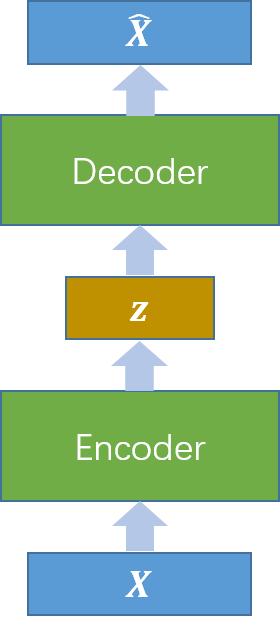
\includegraphics[width=0.3\textwidth]{VAE.png}
  \caption{VAE的简化图}
  \label{fig:vae}
  %\vspace*{-0.6em}
\end{figure}
VAE的主要结构如图~\ref{fig:vae}所示。一个训练好的VAE可以在给定一个特定维度的输入向量之后,生成一个特定的结果(如一幅图像)。在训练的过程中,需要将现有的数据输入VAE中给定数据$\bm X$($\bm X$可以是用向量表示的任意数据)编码成一个低维的表征向量$\bm z$,然后再从$\bm z$出发,重构出$\bm{\hat X}$,使得$\bm X$和$\bm{\hat X}$越接近越好。VAE最根本的目标在于最大化从$\bm z$重构$\bm X$的概率,目标如下所示:
\begin{equation}
\label{eq:baseeq}
%\vspace*{-0.6em}
P(\bm X)=\int P(\bm X|\bm z, \theta)P(\bm z)d\bm z.
\end{equation}

在生成的过程中,随机选取一个向量$\bm r$,从图~\ref{fig:vae}所示的模型中的$\bm z$处输入,即可从$\bm{\hat X}$得到一个生成的数据。\par

实际上,对于特定数据$\bm X$,只会在特征空间中对应特定的$\bm z$,换句话说,对于绝大多数$\bm z$,都是无法生成对应的$\bm X$的,即对于绝大多数$\bm z$,$P(\bm X|\bm z, \theta)$会接近于0。在训练的过程中,模型需要找到这个特定的$\bm z$,使得$P(\bm X|\bm z, \theta)$尽量地大,并从中计算$P(\bm X)$。这意味着我们需要一个新的函数$Q(\bm z|\bm X)$,它可以通过输入$\bm X$的值,给出一个可能产生$\bm X$的$\bm z$值的分布。模型会使得Q值下可能的$\bm z$的空间会大大地小于先前$P(\bm z)$下可能的所有$\bm z$的空间。通过这个方法,可以改为计算$E_{\bm z\sim Q}P(\bm X|\bm z)$,计算会变得更为容易。然而,如果$\bm z$不服从$\mathcal N(\bm 0, \bm I)$,而是从一个随机的概率分布$Q(\bm z)$中采样的,那么这并不能帮助优化$P(\bm X)$。VAE需要首先把$E_{\bm z\sim Q}P(\bm X|\bm z)$和$P(\bm X)$联系起来。\par

$E_{\bm z\sim Q}P(\bm X|\bm z)$和$P(\bm X)$之间的关系是变分贝叶斯方法的基础之一。从$P(\bm X|\bm z)$和$Q(\bm z)$之间的Kullback-Leibler散度($\mathcal{KL}$散度,即$\mathcal D$)的定义开始,对于一些任意$Q$:
\begin{equation}
\label{eq:KL}
%\vspace*{-0.6em}
\mathcal D{[Q(\bm z)||P(\bm z|\bm X)]} = E_{\bm z\sim Q}{[\log Q(\bm z)-\log P(\bm z|\bm X)]}
\end{equation}
通过将应用贝叶斯准则应用于$P(\bm z|\bm X)$,可以将$P(\bm X)$和$P(\bm X|\bm z)$引入公式~\ref{eq:KL}:
\begin{equation}
\label{eq:KL1}
%\vspace*{-0.6em}
\mathcal D{[Q(\bm z)||P(\bm z|\bm X)]} = E_{\bm z\sim Q}{[\log Q(\bm z)-\log P(\bm X|\bm z) - \log P(\bm z)]} + \log P(\bm X)
\end{equation}
在这里,$\log P(\bm X)$被从期望中提出,是因为它不依赖于$\bm z$。将等式中$-\log P(\bm X|\bm z) - \log P(\bm z)$改写成$\mathcal{KL}$散度的形式后得到:
\begin{equation}
\label{eq:KL2}
%\vspace*{-0.6em}
\log P(\bm X) - \mathcal D{[Q(\bm z)||P(\bm z|\bm X)]} = E_{\bm z\sim Q}{[\log P(\bm X|\bm z)]} - \mathcal D{[Q(\bm z)||P(\bm z)]}
\end{equation}
这里,需要注意的是,$\bm X$是固定的,$Q$可以是任何分布,而不仅仅是一个将$\bm X$映射到可以产生$\bm X$的$\bm z$的分布。由于现在需要推导$P(\bm X)$,所以构造一个取决于$\bm X$的$Q$很有必要,而且,这个$Q$要使$\mathcal D{[Q(\bm z)||P(\bm z|\bm X)]}$变小:
\begin{equation}
\label{eq:vae_key}
%\vspace*{-0.6em}
\log P(\bm X) - \mathcal D{[Q(\bm z|\bm X)||P(\bm z|\bm X)]} = E_{\bm z\sim Q}{[\log P(\bm X|\bm z)]} - \mathcal D{[Q(\bm z|\bm X)||P(\bm z)]}
\end{equation}
这个等式相当于VAE的核心,所以这里用两句话解释一下它的内容。等式左边有VAE想要最大化的值:$\log P(\bm X)$(加上一个误差项$\mathcal D{[Q(\bm z|\bm X)||P(\bm z|\bm X)]}$,它使得$\bm Q$产生可以重构给定$\bm X$的$\bm z$)。而对于等式右边,VAE可以通过选择正确的$Q$来进行随机梯度上升优化(然而不同的$Q$对于结果的影响并不明显)。值得注意的是,VAE模型在这里突然采用了一种看起来像自动编码器(autoencoder,即AE)的形式(尤其是公式~\ref{eq:vae_key}的右边),因为$Q$将$\bm X$编码为$\bm z$,并且$P$对其进行“解码”以重建$\bm X$。\par

VAE的目标就是最大化公式~\ref{eq:vae_key}。首先看$\mathcal D{[Q(\bm z|\bm X)||P(\bm z)]}$。由于$Q$和$P$的具体分布对于结果并没有很大影响,这里假设$Q$和$P$都是高斯分布,即$Q=\mathcal N(\bm {\mu_0}|\bm {\Sigma_0})$,$P=\mathcal N(\bm {\mu_1}|\bm {\Sigma_1})$。这里为了简化问题,假设$P$的分布是标准高斯分布,即$\mathcal N(\bm 0|\bm I)$。那么公式~\ref{eq:vae_key}中$\mathcal{KL}$散度的部分即可改写为$\mathcal D{[\mathcal N(\bm \mu(\bm X)|\bm \Sigma(\bm X))||\mathcal N(\bm 0|\bm I)]}$。这部分可以通过如下过程进行简化:
\begin{equation}
\label{eq:KL_infer}
%\vspace*{-0.6em}
\begin{aligned}
  &\mathcal D{[\mathcal N(\bm \mu(\bm X)|\bm \Sigma(\bm X))||\mathcal N(\bm 0|\bm I)]} \\
= &\int {[\frac{1}{2}\log \frac{1}{|\bm \Sigma(\bm X)|} - \frac{1}{2}(\bm z - \bm \mu (\bm X))^\top \bm \Sigma(\bm X)^{-1}(\bm z - \bm \mu (\bm X)) + \frac{1}{2}\bm z^\top\bm z]}\times \mathcal N(\bm \mu(\bm X)|\bm \Sigma(\bm X))dz \\
= &\frac{1}{2}\log \frac{1}{|\bm \Sigma(\bm X)|}-\frac{1}{2}\mathrm{tr}\{E{[(\bm z - \bm \mu (\bm X)(\bm z - \bm \mu (\bm X))^\top]\bm \Sigma(\bm X)^{-1}}\} + \frac{1}{2}E{[\bm z^\top\bm z]} \\
= &\frac{1}{2}\log \frac{1}{|\bm \Sigma(\bm X)|}-\frac{1}{2}d + \frac{1}{2}\bm \mu (\bm X)^\top\mu (\bm X) + \frac{1}{2}\mathrm{tr}\{\bm \Sigma(\bm X)\} \\
= &-\frac{1}{2}{[\log |\bm \Sigma(\bm X)| + d - \bm \mu (\bm X)^\top\mu (\bm X) - \mathrm{tr}\{\bm \Sigma(\bm X)\}]}.
\end{aligned}
\end{equation}
\par
之后,对于公式~\ref{eq:vae_key}中$E_{\bm z\sim Q}{[\log P(\bm X|\bm z)]}$的部分,需要用到重参数化的技巧。对这部分进行估计可以通过对$\bm z$进行采样。但是,若要取得好的效果,则需要对$\bm z$进行大量的采样,这将是一个非常大的开销。所以,在实际优化过程中,只是对$\bm z$进行一次采样,将这次采样作为对真实分布的估计。目标函数优化的过程中需要用到梯度下降,但是,这就造成了一个严重的问题,那就是,如果采用对$\bm z$采样的方式来优化目标函数,那么最终的梯度和$\mathcal{KL}$散度部分将会没有任何联系,也就是说,用梯度下降的方法将无法优化整个目标函数。这里就需要用到重参数化的方法。\par
\begin{figure}[h]
  \centering
  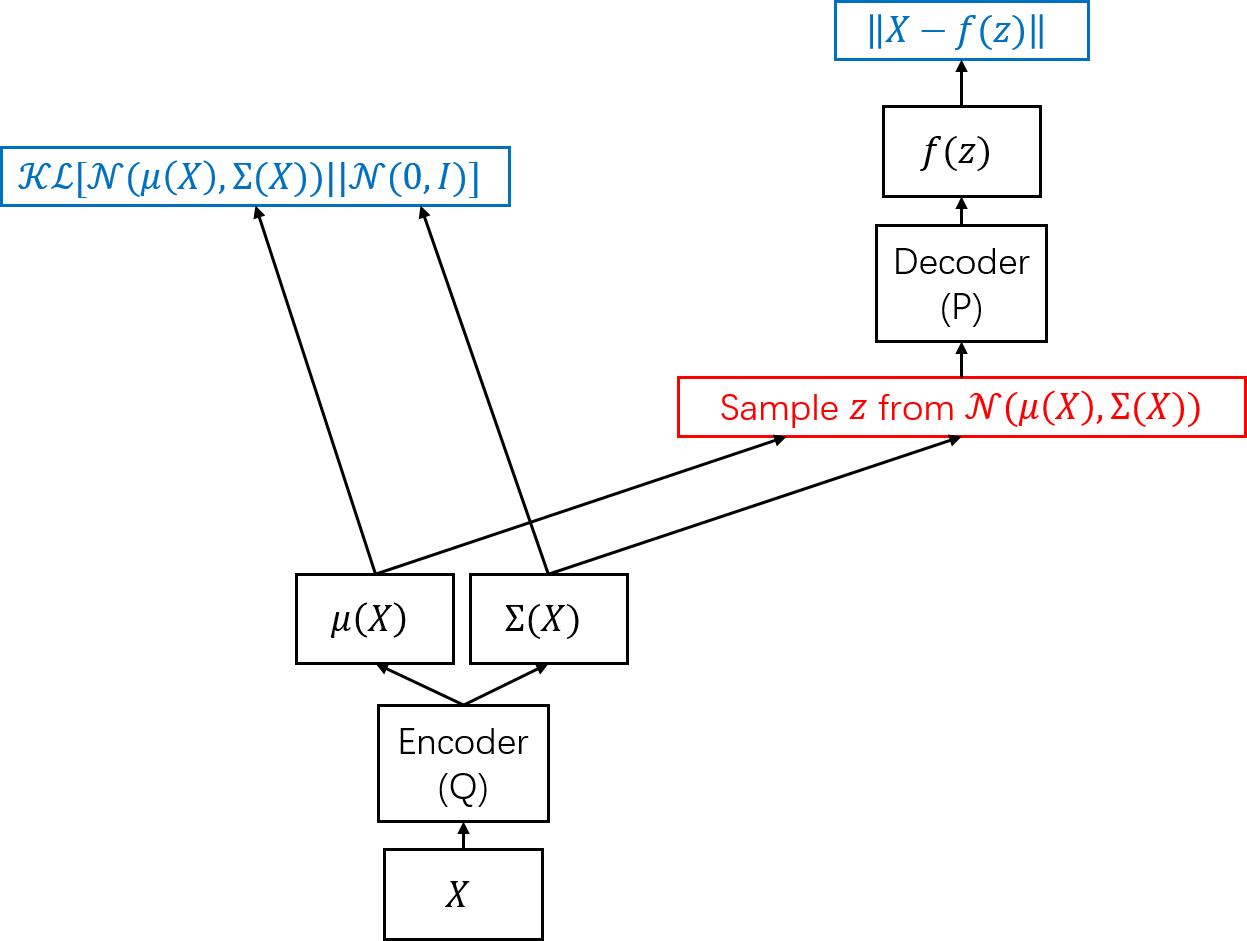
\includegraphics[width=0.7\textwidth]{noreparam.png}
  \caption{直接采样$\bm z$}
  \label{fig:noreparam}
  %\vspace*{-0.6em}
\end{figure}
\begin{figure}[h]
  \centering
  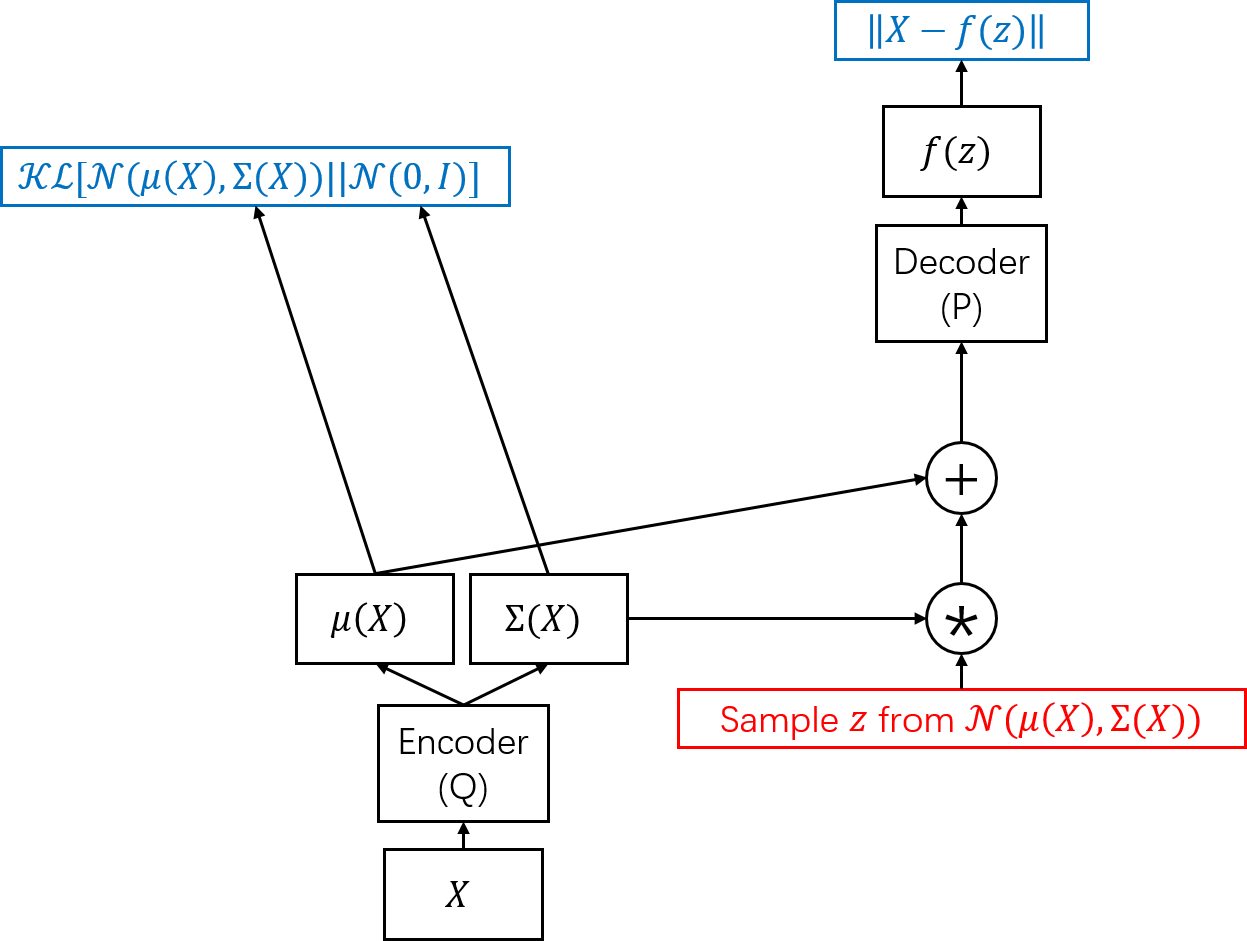
\includegraphics[width=0.7\textwidth]{reparam.png}
  \caption{采用重参数化}
  \label{fig:reparam}
  %\vspace*{-0.6em}
\end{figure}
重参数化即在采样时,先从标准正态分布$\mathcal N(\bm 0|\bm I)$中采样一个随机向量$\bm \epsilon$,然后通过$\bm \epsilon \bigodot \bm \Sigma(\bm X) + \bm \mu (\bm X)$获得采样得到的$\bm z$,其中$\bigodot$表示向量之间的按位乘法。这样,$\bm z$就和$\bm \Sigma(\bm X)$和$\bm \mu (\bm X)$有了联系,梯度的传递就可以达到$\mathcal{KL}$散度部分了。\par

对于不同的数据,$P(\bm X|\bm z)$对应不同的分布,若数据是实数数据,那么对应的是高斯分布,若数据是0-1数据,那么对应的是伯努利分布。以下讨论最简单的情况,即采用多层感知机(multi-layer perceptrons,以下简称MLP)构建VAE。\par

对于高斯分布的情况,在图~\ref{fig:reparam}中Decoder部分需要从$\bm z$再采样$\bm X$来重构$\bm X$。$\log P(\bm X|\bm z)$通过以下方式计算:
\begin{equation}
  \begin{gathered}
  %\vspace*{-1em}
  \label{eq:gaussian}
\log P(\bm X|\bm z) = \log \mathcal N(\bm X; \bm \mu(\bm z), \bm \Sigma(\bm z)) \\
\bm \mu(\bm z) = \bm {W_1}\bm h + \bm {b_1} \\
\log \bm \Sigma(\bm z) = \bm {W_2}\bm h + \bm {b_2} \\
\bm h = f(\bm {W_3}\bm z + \bm {b_3}),
  \end{gathered}
\end{equation}
其中,$\bm {W_1}$、$\bm {W_2}$、$\bm {W_3}$、$\bm {b_1}$、$\bm {b_2}$和$\bm {b_3}$都是全连接层的参数,$f$是全连接层后的激活函数。\par

对于伯努利分布的情况,图~\ref{fig:reparam}中Decoder部分就是MLP,$\log P(\bm X|\bm z)$通过以下方式计算:
\begin{equation}
  \begin{gathered}
  %\vspace*{-1em}
  \label{eq:bernoulli}
\log P(\bm X|\bm z) = \sum \bm {X_i}\log\bm {\hat X_i} + (1-\bm {X_i})\log(1 - \bm {\hat X_i}) \\
\bm {\hat X_i} = sigmoid(\bm {W_5}(\bm {W_4}\bm z + \bm {b_4}) + \bm {b_5}),
  \end{gathered}
\end{equation}

\section{doc2vec模型}
doc2vec模型是一种学习文本表征向量的模型,通过学习文本中不同单词的分布情况得到整段文本的表征向量。\par
doc2vec模型基于word2vec模型——一种单词表征学习模型。word2vec模型如图~\ref{fig:word2vec}所示。word2vec利用一个滑动窗口扫过整个文本,每次取窗口中的所有单词的表征向量进行更新,图~\ref{fig:word2vec}中CBOW模型的目标为最大化公式~\ref{eq:word2vec1},

% \begin{figure}[h]
%   \centering
%   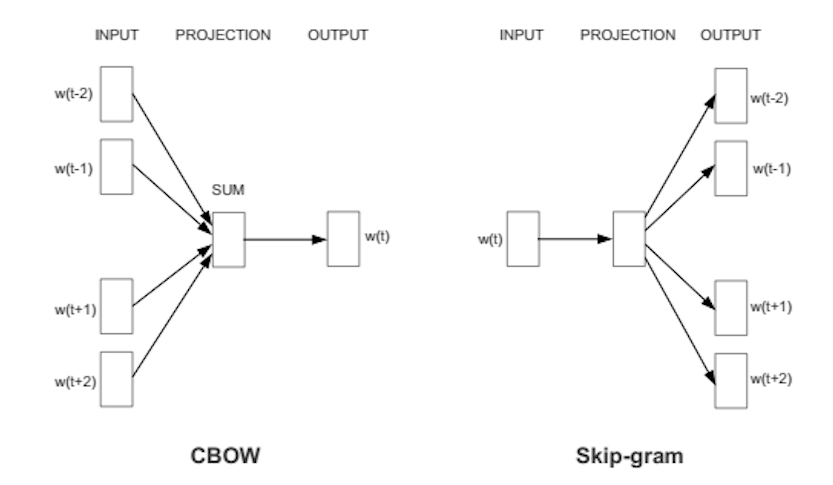
\includegraphics[width=1\textwidth]{word2vec.png}
%   \caption{word2vec的两种模式}
%   \label{fig:word2vec}
%   %\vspace*{-0.6em}
% \end{figure}
\begin{figure}[t]

  \begin{subfigure}[t]{0.5\linewidth}  
    \centering
    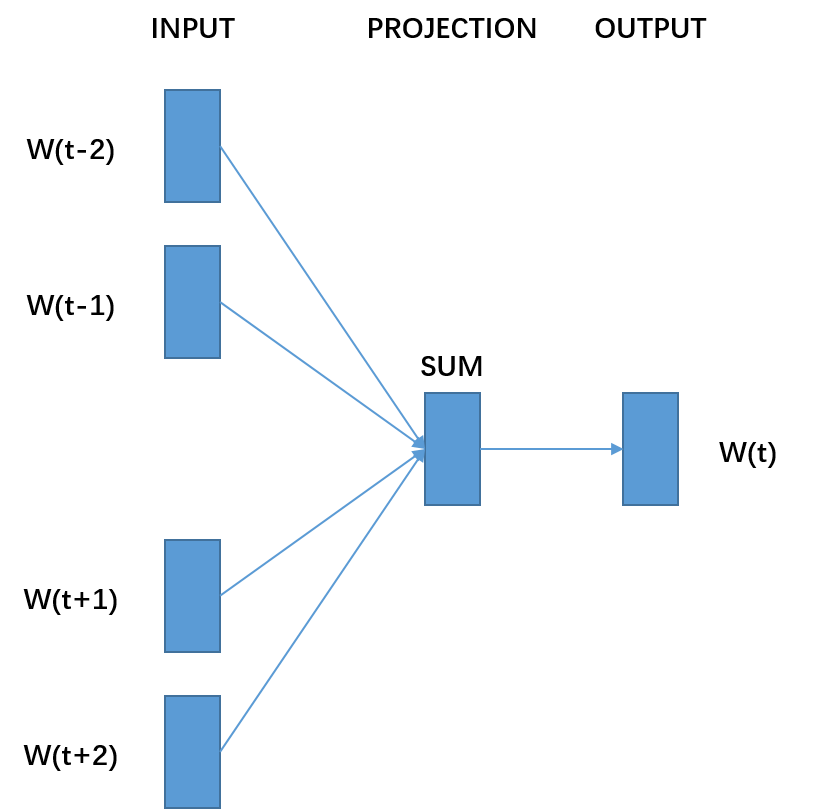
\includegraphics[width=6.5cm]{cbow.png}

    \caption{CBOW}
    \label{fig:jaccard}
  \end{subfigure}
  \begin{subfigure}[t]{0.5\linewidth}  
    \centering
    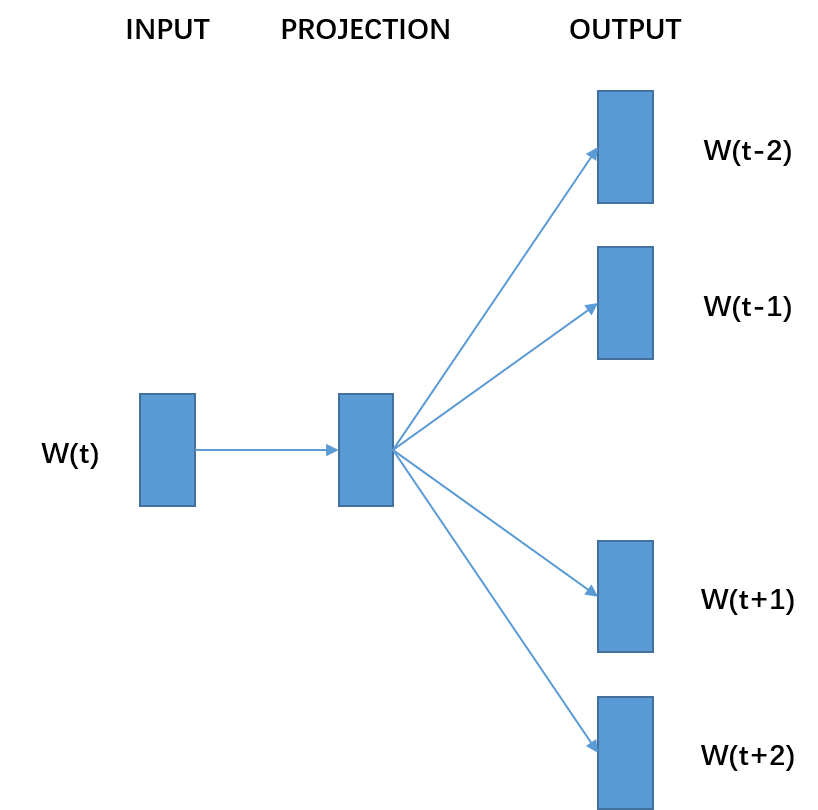
\includegraphics[width=6.5cm]{sg.png}

    \caption{Skip-gram}
    \label{fig:f1}
    
  \end{subfigure}  
  
  \caption{word2vec的两种模式}
  \label{fig:word2vec}
%     \vspace{-1em}
\end{figure}

\begin{equation}
  \label{eq:word2vec1}
  \frac{1}{T}\sum_{t=k}^{T-k}\log p(\bm {w_k}|Context(\bm {w_k})),
\end{equation}
其中$T$为整段文本的单词总数,$k$为滑动窗口一侧的大小,$\bm {w_i}$为第$i$个单词的表征向量,$Context(\bm {w_k})$是单词$k$的上下文中单词的向量。图~\ref{fig:word2vec}中Skip-gram模型的目标为最大化公式~\ref{eq:word2vec2},
\begin{equation}
  \label{eq:word2vec2}
  \frac{1}{T}\sum_{t=k}^{T-k}\log p(Context(\bm {w_k})|\bm {w_k}),
\end{equation}
最大化公式~\ref{eq:word2vec1}和公式~\ref{eq:word2vec2}就是最大化在每个窗口中单词共同出现的概率。\par

与word2vec模型类似,doc2vec模型也有两种模式,如图~\ref{fig:doc2vec}所示,分别为PV-DM和PV-DBOW。\par

% \begin{figure}[h]
%   \centering
%   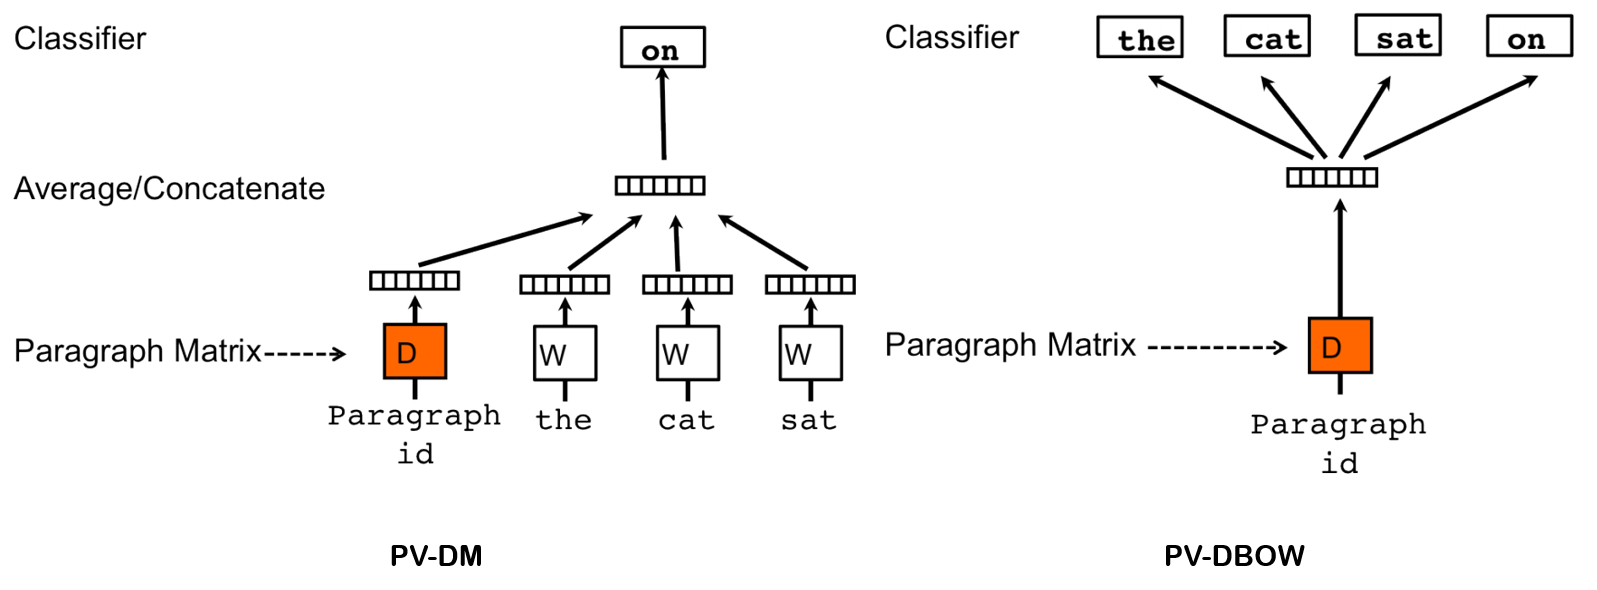
\includegraphics[width=1\textwidth]{doc2vec.png}
%   \caption{word2vec的两种模式}
%   \label{fig:doc2vec}
%   %\vspace*{-0.6em}
% \end{figure}

\begin{figure}[t]
  \begin{subfigure}[t]{0.5\linewidth}  
    \centering
    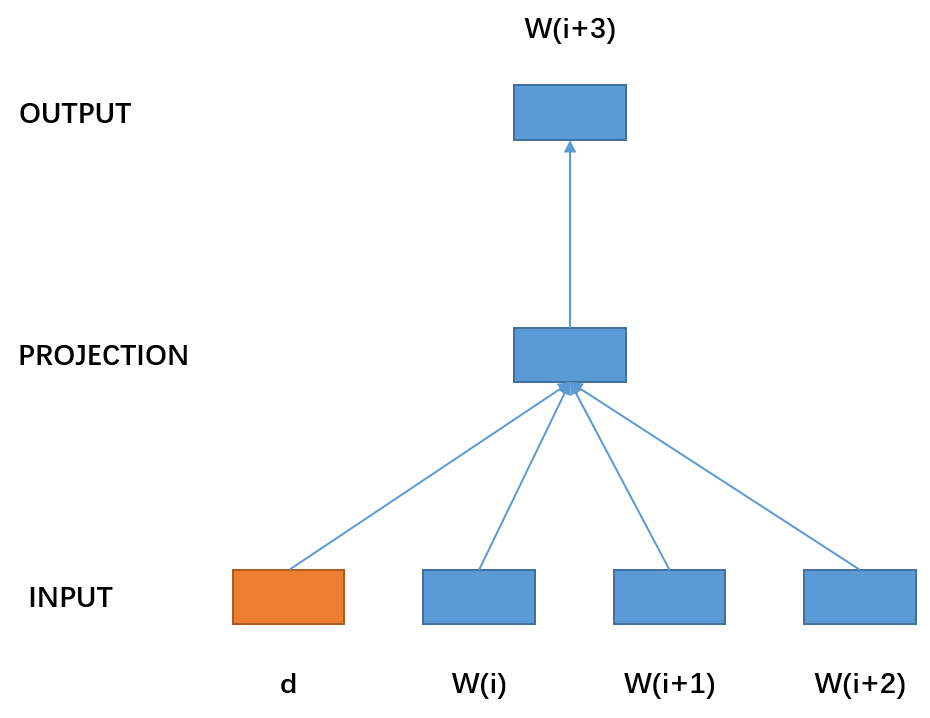
\includegraphics[width=6.5cm]{dm.png}

    \caption{PV-DM}
    \label{fig:jaccard}
  \end{subfigure}
  \begin{subfigure}[t]{0.5\linewidth}  
    \centering
    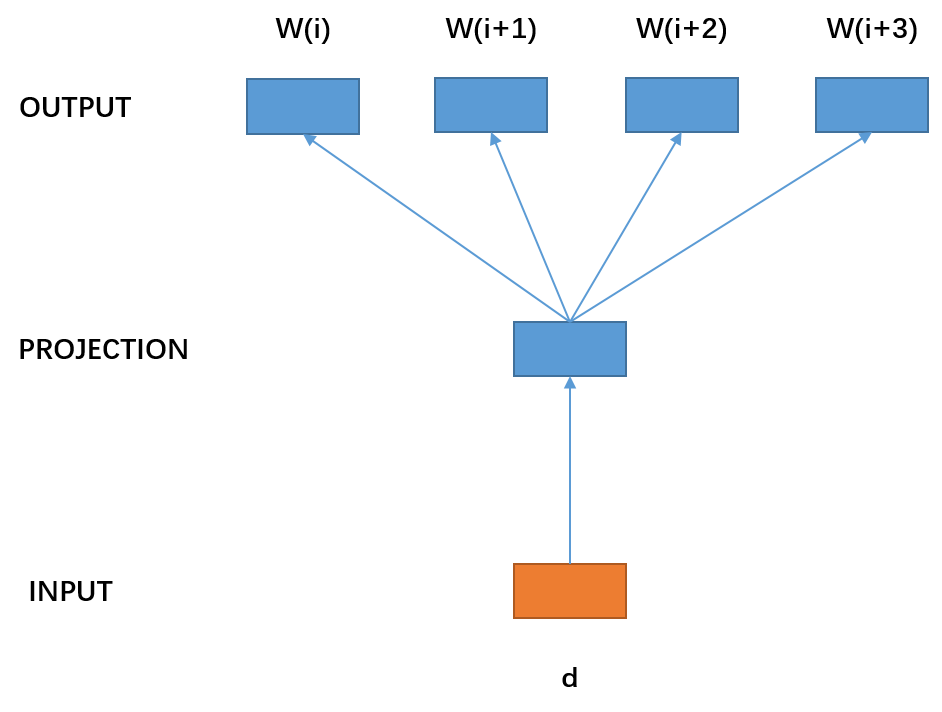
\includegraphics[width=6.5cm]{dbow.png}

    \caption{PV-DBOW}
    \label{fig:f1}
    
  \end{subfigure}  
  
  \caption{doc2vec的两种模式}
  \label{fig:doc2vec}
%     \vspace{-1em}
\end{figure}

doc2vec模型相比于word2vec模型,加入了一个文本标签向量。文本标签向量在训练时与其他单词向量一起训练,但是与其他单词有一点不同,即文本标签向量在每个窗口训练时都会更新。PV-DM模型类似于word2vec的CBOW模型,PV-DBOW类似于word2vec的Skip-gram模型。\par


\begin{figure}[h]
  \centering
  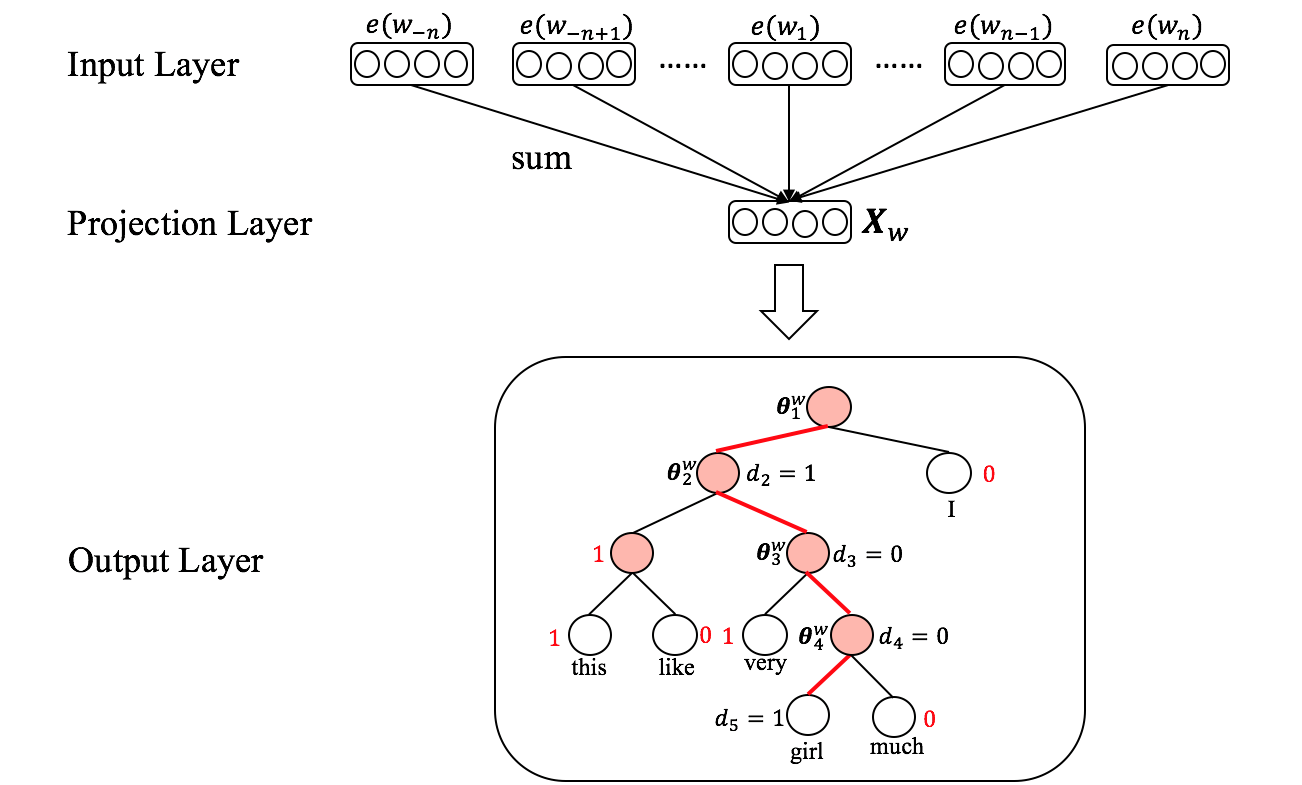
\includegraphics[width=0.7\textwidth]{hierarchical_softmax.png}
  \caption{hierarchical softmax}
  \label{fig:hsoftmax}
  %\vspace*{-0.6em}
\end{figure}

word2vec模型在学习时有两种优化方式,一是层次softmax~\autocite{morin2005hierarchical},二是负采样~\autocite{mikolov2013distributed}。\par
层次softmax方法基于哈夫曼树。如图~\ref{fig:hsoftmax}所示,哈夫曼树的每个节点都对应一个向量,叶节点对应的是单词向量,而内部节点对应的是一个辅助向量$\bm {\theta^w_i}$,映射层中$\bm x_w$为输入层各个向量的和。在层次softmax中,每一层节点都相当于一次逻辑回归的二分类。从根节点到达一个叶节点的路径,即为路径上每个公式~\ref{eq:word2vec1}中$p(\bm {w_k}|\bm {w_{t-k}}, ..., \bm{w_{t+k}})$即为从根节点开始,到$\bm {w_k}$对应的叶节点路径上二分类概率之积。以图~\ref{fig:hsoftmax}中单词girl为例,从根节点出发,到girl的节点,经过了$d_2$、$d_3$、$d_4$、$d_5$四个节点,每次二分类的概率分别为:
\begin{equation}
  \label{eq:hsoftmax}
  \begin{gathered}
  p(d_2|\bm {x_w}, \bm {\theta_1^w}) = \sigma(\bm {x_w}^\top \bm{\theta_1^w})\\
  p(d_3|\bm {x_w}, \bm {\theta_2^w}) = 1-\sigma(\bm {x_w}^\top \bm{\theta_2^w})\\
  p(d_4|\bm {x_w}, \bm {\theta_3^w}) = 1-\sigma(\bm {x_w}^\top \bm{\theta_3^w})\\
  p(d_5|\bm {x_w}, \bm {\theta_4^w}) = \sigma(\bm {x_w}^\top \bm{\theta_4^w}),
  \end{gathered}
\end{equation}
从而$p(\bm {girl}|Context(girl)) = \prod_{i=2}^5 p(d_i|\bm {x_w}, \bm {\theta_{i-1}^w})$,其中$\sigma$是sigmoid函数。Skip-gram的计算方式与CBOW类似,由于本文采用doc2vec的PV-DM模型,与word2vec的CBOW模型接近,所以此处对于Skip-gram的计算方式不再赘述。\par

在负采样的优化方法中,目标函数变为
\begin{equation}
\label{eq:neg}
p(\bm {w_k}|Context(\bm {w_k})) = \prod_{u\in {k}\bigcup Neg(k)}{[\sigma(\bm{x_w}^\top \bm{w_u})]^T_k(u)\cdot{[1-\sigma(\bm{x_w}^\top \bm{w_u})]^{[1-T_k(u)]}}},
\end{equation}
其中,$Neg(k)$是对单词$k$进行负采样得到的负样本集合;$u$是对单词$k$采样得到的样本单词的序号;$T_k(u)$是一个标志量,若$u=k$,则$T_k(u)=1$,若$u\ne k$,则$T_k(u)=0$。

\section{本章小结}
本章介绍了与HAVAE模型相关的一些预备知识。\par
本章首先介绍了本文中主要用到的一些符号;之后介绍了一些韵律文本相关知识,包括单韵和隔行韵等韵律模式、模型用到的音素字母表等;之后提出了韵律特征提取问题和特征融合问题;之后简单介绍了VAE的原理及其训练过程;最后介绍了doc2vec模型。\par

\chapter{利用层次注意力机制的VAE模型} \label{chpt:model}

本文提出的模型的结构如图~\ref{fig:model}所示。模型包括两个主要模块,分别是特征提取模块和特征融合模块。特征提取模块用于将输入内容编码成分布式的韵律和语义向量。输入内容包括原始的韵律文本,以及歌词的韵律形式。特征融合模块用于有效地融合语义信息和韵律特征。最终学习到的表征向量可以用于许多任务中,例如本文实验部分将提到的歌词预测任务。\par
\begin{figure*}[h]
  \centering 
  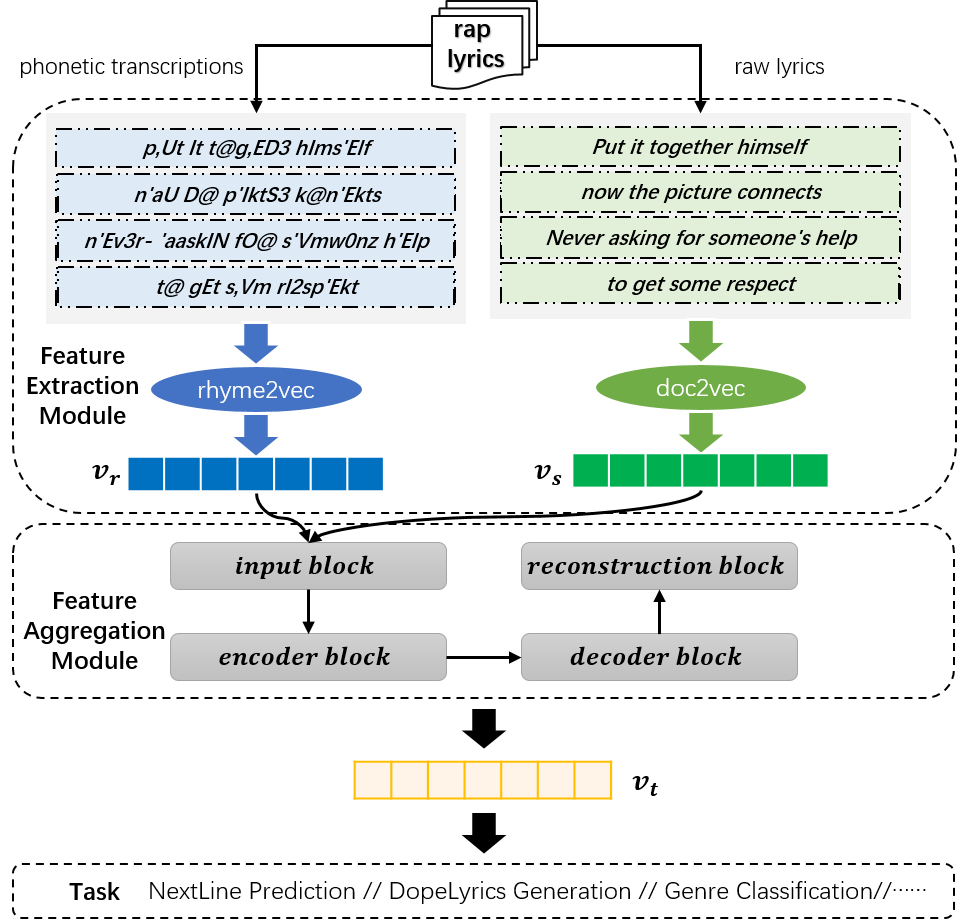
\includegraphics[width=12cm]{model.png}
  \caption{HAVAE的结构}
  \label{fig:model}
\end{figure*}

\section{特征提取模块} \label{sec:fe}
特征提取模块(如图~\ref{fig:model}所示)用来获取适当细化的特征。特征提取模块由两部分组成,分别是韵律部分和语义部分。\par

\subsection{韵律部分}
本节将介绍一个用于解决问题~\ref{p:rhyme}的方法。此方法称为rhyme2vec。图~\ref{fig:rhyme2vec}展示了由给出的韵律文本获取韵律表征向量$\bm {v_r}$的完整过程。\par

\begin{figure}[h]
  \centering
  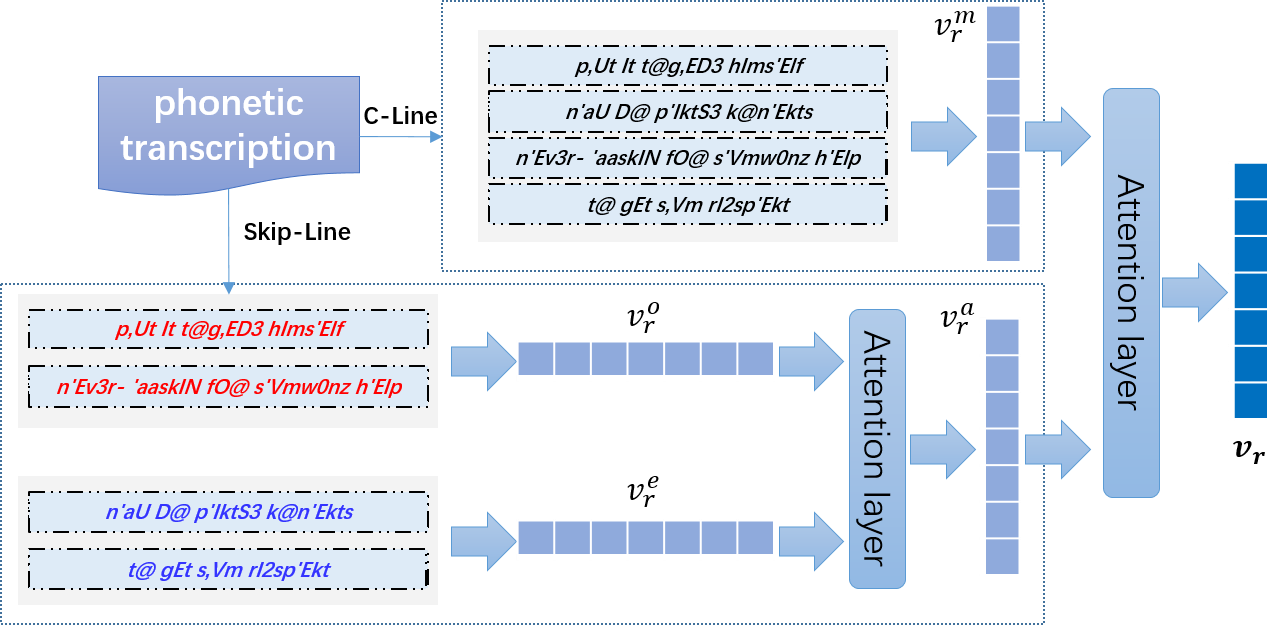
\includegraphics[width=1\textwidth]{rhyme.png}
  \caption{rhyme2vec的结构}
  \label{fig:rhyme2vec}
\end{figure}
每首说唱歌曲包括三个韵律段。首先,将每个音素映射成一个单独的向量,记为$\bm{v_p}$。受~\autocite{quoc2014distributed}学习文本的想法的启发,每个韵律段都被赋予了一个段向量,记作$\bm {v_b}$。一个韵律段的向量记为$\bm {v_r^b} (\bm b \in \{\bm{m, o, e}\})$。$\bm {v_r^b}$定义为该韵律段中所有音素向量和段向量的和,即$\bm {v_r^b}=\sum\bm{v_{p}}+\bm{v_b}$。利用一个固定长度的滑动窗口将一个韵律段划分为若干个小韵律段,模型通过最大化每个小韵律段中各个音素共同出现在该大韵律段中的概率来训练出所有的$\bm {v_p}$和$\bm{v_b}$。\par

模型的损失函数写作:
\begin{equation}
%\vspace*{-0.6em}
\mathcal L_{\bm r} =\frac{1}{3N}\times \sum_{i=1}^{3N}\frac{1}{{n_i}-2w}\times \sum\limits_{j=w}^{n_i-w}\log P(\bm {v_p^{j,i}}|\bm {(v_p^{j-w,i}}: \bm {v_p^{j+w,i}}, \bm {v_b^{i}})),
\end{equation}
其中,$n_i$为第$i$个韵律段中音素的个数;$w$是滑动窗口一边的大小;$\bm {v_p^{j, i}}$是第$i$个韵律段中第$j$个音素对应的向量;$\bm {v_b^{i}}$是第$i$个韵律段的段向量。为了提高训练效率和改善训练效果,本文采用了负采样的方法进行训练。目标函数写为:
\begin{equation}
%\vspace*{-0.6em}
\bm{\mathcal{L}_r}=\bm{\mathcal{L}_{r,pos}}- k \times \bm{\mathcal{L}_{r,neg}},
\end{equation}
其中,$k$是每个正样本对应的负样本的个数。\par

需要注意的是,为了学习单韵模式,本文提出了连续行学习模型记作C-Line(图~\ref{fig:rhyme2vec}的上半部分)。在C-Line中,整段输入歌词的韵律形式$\bm{L_r^m}$作为输入内容,利用上述方法,从对应的音素向量和段向量中计算得到一个分布式向量$\bm{v_r^m}$,即为单韵韵律的表示向量,对应于上述方法中的$\bm {v_r^b}$。\par

本文用$\bm {v_r^a}$指代隔行韵模式的表示向量。由于单韵和隔行韵在一段韵律文本中的重要性不同,本文引入了注意力层来为$\bm {v_r^m}$和$\bm {v_r^a}$赋予不同的权重,以平衡单韵模式和隔行韵模式在最终韵律表示向量中所占权重。注意力层的输入为一个由若干列向量组成的矩阵$\bm{\mathcal{H}}$,注意力层的计算方法如下所示:
\begin{equation}
  \begin{gathered}
  %\vspace*{-1em}
  \label{eq:att}
  Attention(\bm {H}) = \sum_{j=0}^{m-1}{\bm{\alpha{_j} h{_j}}}\\
  \alpha_i= \frac{exp\left( \bm{\hat{h}{_i}^{\top } \hat{h}_{c}}\right) }{\sum_{j=0}^{m-1}{exp\left( \bm {\hat{h}{_j}^\top \hat{h}_{c}} \right) } }\\
\bm{\hat{h}_i}= tanh(\bm {W_u}\bm{h_i}+\bm{b_u}),
  \end{gathered}
\end{equation}
其中,$m$是输入矩阵$\bm{\mathcal{H}}$的列数;$\bm {h_i}$是$\bm{\mathcal{H}}$的第$i$列($0 \leq i \leq m-1$);$\bm {\hat{h}_i} $是由$\bm h_i$通过$tanh$函数计算出的一个隐含向量;$\alpha_i$是由$\bm {\hat{h}_i}$和一个随机初始化的上下文向量$\bm{\hat{h}_{c}}$计算出的权重;$\bm {W_u}$和$\bm {b_u}$是随机初始化后,在训练中训练出的参数矩阵。最终的融合向量$\bm t$是所有$\bm {h_i}$的加权和。在融合$\bm {v_r^m}$和$\bm {v_r^a}$的注意力层中,$\bm{\mathcal{H}}$由$\bm {v_r^m}$和$\bm {v_r^a}$两个列向量组成,即$\bm{\mathcal{H}=[\bm {v_r^m}; \bm {v_r^a}}]$。$\bm {v_r}= \bm{t}$是最终的韵律表征向量。\par

需要注意的是,为了学习单韵模式,本文提出了跳行学习模型记作Skip-Line(图~\ref{fig:rhyme2vec}的下半部分)。在Skip-Line中,不同于C-Line,歌词的韵律形式首先被分为奇数行段(包括所有的奇数行,记作$\bm{L_r^o}$)和偶数行段(包括所有的偶数行,记作$\bm{L_r^e}$)。$\bm{v_r^o}$和$ \bm{v_r^e}$是以和$\bm{v_r^m}$同样的方法,分别从$\bm{L_r^o}$和$\bm{L_r^e}$计算得到的分布式向量。另外,与融合单韵模式和隔行韵模式类似,本文在$\bm{v_r^o}$和$\bm{v_r^e}$之后用了一个注意力层,其中,$\bm{\mathcal{H}}$由$\bm{v_r^o}$和$\bm{v_r^e}$两个列向量组成。\par

最终,$\bm {L}$的韵律的表征向量通过rhyme2vec方法得到,即
\begin{equation}
  \begin{gathered}
  %\vspace*{-1em}
  \label{eq:vr}
  \bm{v_r}=Att([\bm {v_r^m}; Attention([\bm{v_r^o}; \bm{v_r^e}])]).
  \end{gathered}
\end{equation}
\par

总的来说,rhyme2vec的算法可以总结为算法~\ref{alg:rhyme2vec}。\par
\begin{algorithm}  
        \caption{rhyme2vec} 
        \label{alg:rhyme2vec} 
        \begin{algorithmic}[1] 
            \Require $\bm {L_r^m}$, $\bm {L_r^o}$, $\bm {L_r^e}$, 窗口大小 $w$, 向量维度 $d$, 负采样数量 $n$
            \Ensure $\bm {v_r}$
                \State $\bm {v_r^m} = \Call{rhymeEmbedding}{\bm {L_r^m}, w, d, n}$ 
                \State $\bm {v_r^o} = \Call{rhymeEmbedding}{\bm {L_r^o}, w, d, n}$ 
                \State $\bm {v_r^e} = \Call{rhymeEmbedding}{\bm {L_r^e}, w, d, n}$ 
                \State $\bm {v_r^a} = \Call{Attention}{{[\bm {v_r^o}, \bm {v_r^e}]}}$ 
                \State $\bm {v_r} = \Call{Attention}{{[\bm {v_r^m}, \bm {v_r^a}]}}$ 
                \State \Return{$v_r$}  
        \end{algorithmic}  
\end{algorithm}  
其中,$\Call{Attention}{a, b}$函数即为公式~\ref{eq:att}。

\begin{algorithm}  
        \caption{rhymeEmbedding} 
        \label{alg:rhymeembedding} 
        \begin{algorithmic}[1]  
        \Require $\bm {L_t}$, 窗口大小 $w$, 向量维度 $d$, 负采样数量 $n$
            \Ensure $\bm {v_t}$
            
              \State $\bm {V_t}, \bm {\theta_t} = \Call{initializeEmbedding}{|\bm {L_t}| + 1, d}$
                \For{each epoch}
                  \For{$i = 1 \to |\bm {L_t}|$}
                      \State $\bm e = \bm 0$
                      \State $\bm x_i = \sum_{k\in \Call{Context}{i}} \bm {V_{t, k}} + \bm {V_{t, 0}}$
                      \For{$j \in \{i\}\bigcup \Call{Neg}{i, n}$}
                          \State $q = \sigma(\bm x_i^\top \bm {\theta_{t, j}})$
                          \State $g = \eta{[T_i(j)-\sigma(\bm {V_{t, j}}^\top \bm {x_i})]}$
                          \State $\bm e = \bm e + g\bm {\theta_{t, j}}$
                          \State $\bm {\theta_{t, j}} = \bm {\theta_{t, j}} + g\bm {x_i}$
                      \EndFor
                      \For{$j \in \Call{Context}{i}\bigcup \{0\}$}
                          \State $\bm V_{t, j} = \bm V_{t, j} + \bm e$
                      \EndFor
  %                     \For{$$}

                  \EndFor
                \EndFor
                \State $\bm {v_t} = \sum_{i = 0}^{|\bm {L_t}|}\bm{V_{t, i}}$
                \State \Return{$\bm {v_t}$} 
        \end{algorithmic}  
    \end{algorithm}  

算法~\ref{alg:rhymeembedding}中,$\Call{initializeEmbedding}{a, b}$用于初始化$a$个维度为$b$的向量,以及$a$个维度为$b$的辅助向量;$\bm {V_t}$和$\bm {\theta_t}$分别为韵律段和其中音素对应的表征向量和辅助向量;$\Call{Context}{i}$函数的输出为以第$i$个音素为中心、大小为$2w+1$的窗口中除了中心音素以外的音素序号。令训练轮数为$ep$,每一轮中,需要以每一个音素为中心,更新窗口中所有音素向量以及该段韵律段的段向量。更新时,需要首先计算更新向量$\bm e$,这个过程需要计算$n+1$次。所以算法~\ref{alg:rhymeembedding}的时间复杂度为$\Theta({ep[9d(n + 1) + 2(2w + 1)d](|\bm {L_t}|-2w)}+d|\bm {L_t}|)$,即$\mathrm{\bm O}(d\cdot ep \cdot(n+w)(|\bm {L_t}|-w))$。

\subsection{语义部分}

为了提取语义特征,本文应用了doc2vec模型~\autocite{quoc2014distributed}。doc2vec是目前性能最优秀的句嵌入模型之一,分为段落向量的分布式记忆模型(the distributed memory model of paragraph vectors,以下简称PV-DM)和段落向量的分布式词袋模型(the distributed bag-of-words version of paragraph vectors,以下简称PV-DBOW)两种模型。实验表明,PV-DM的性能通常优于PV-DBOW。\par

本文采用了PV-DM来学习$\bm {L}$的语义向量,即$\bm {v_s}$。本文选择了负采样的方式来训练doc2vec模型。在段落的级别上,本文将连续的几行看作一个段落;在歌曲的级别上,我们将整个歌曲看作一个段落。\par

\section{特征融合模块} \label{utm}

\begin{figure}[t]
  \centering
  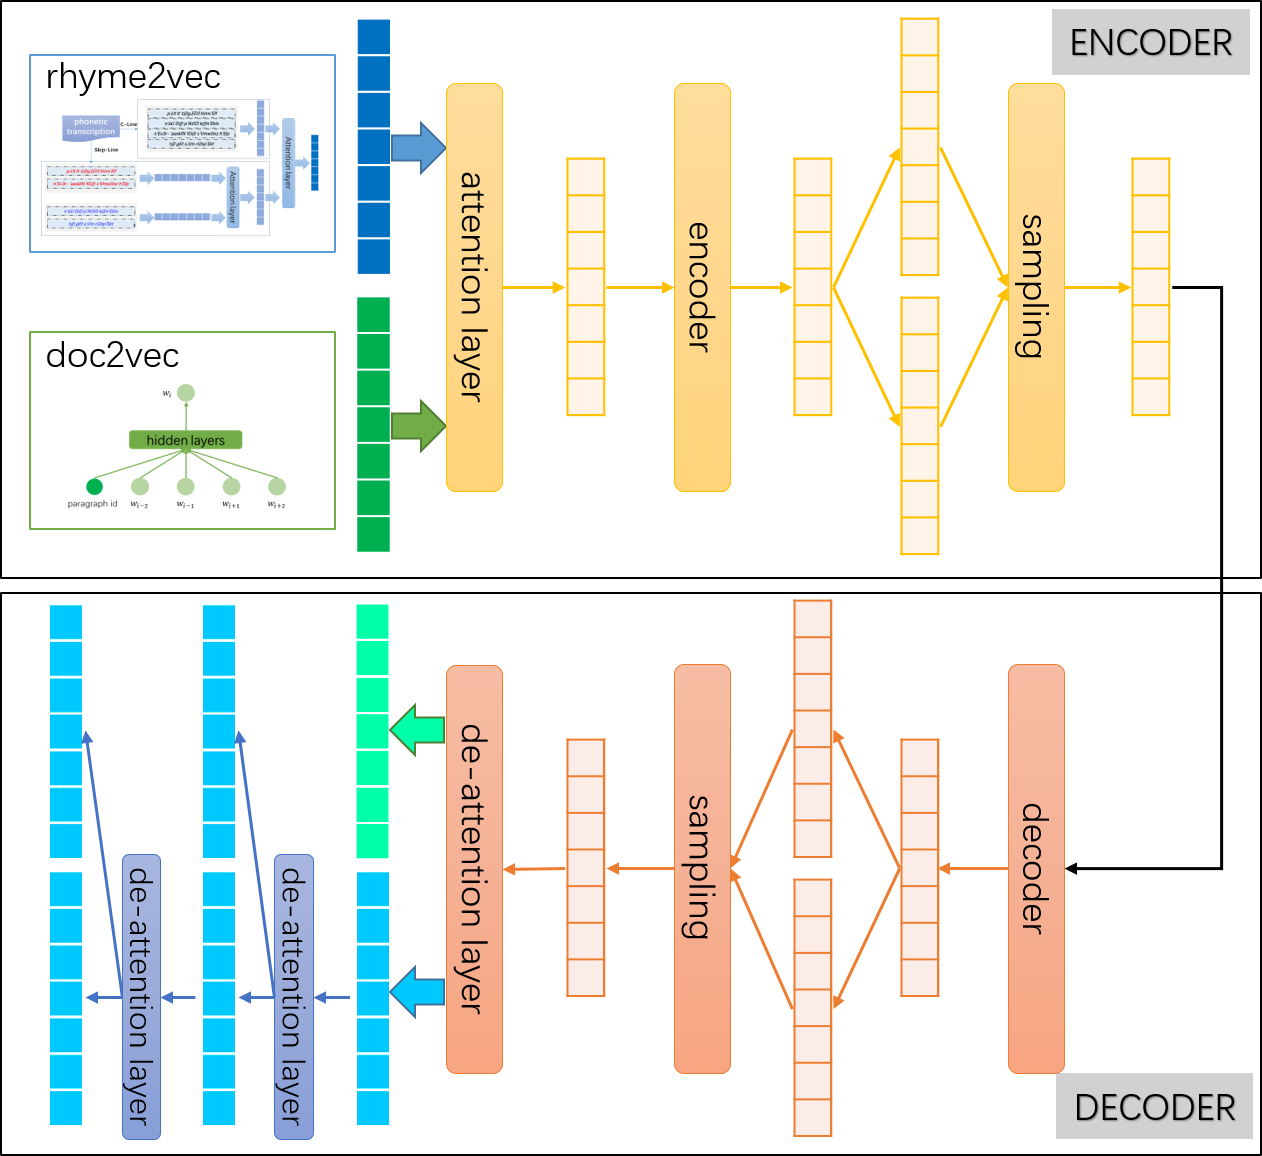
\includegraphics[width=1\textwidth]{HAVAE.png}
  \caption{特征融合模块的结构}
  \label{fig:aggregation}
  %\vspace*{-0.6em}
\end{figure}

特征融合模块用于解决问题~\ref{p:all},是本文所提出的模型的核心部分。这一部分,本文设计了一个通过融合韵律和语义信息来得出韵律文本表征向量的VAE网络。此外,模型还引入了注意力机制来平衡韵律部分和语义部分的重要性。特征融合模块的结构如图~\ref{fig:aggregation}所示,其中包括三个主要的阶段,即输入阶段、编码阶段和解码阶段。\par

\subsection{输入阶段}
在输入阶段,如图~\ref{fig:aggregation}顶部所示,我们用前文提到的注意力层来处理输入数据。通过特征提取模块得到的韵律信息和语义信息的表征向量$\bm{v_r}$和$\bm{v_s}$作为输入。注意力层的输出向量$\bm v$将作为后面的阶段的输入。\par

\subsection{编码阶段}
在编码阶段,首先是若干编码层,每个编码层都是一个全连接层。全连接层的计算公式为 $\bm{h_{i+1}}=tanh(W_i \bm{h_i}+b_i)(1 \leq i \leq k)$,其中$k$是编码层的个数,$tanh$是每个全连接层的激活函数。将$\bm v$输入全连接层后,得到一个隐含向量$u$。VAE网络的目标在于学习隐含向量$\bm z$,使得$\bm z$可以尽可能多地保留$\bm v$的信息。本文从$\bm u$学习到$\bm z$的期望向量和方差对数向量。令$\bm{\mu_z}$为$\bm z$的期望向量,$\log\bm{\sigma_z^2}$为$\bm z$的方差对数向量。假设$\bm z$服从${\mathcal{N}(\bm {\mu_z},\bm{\sigma_z^2})}$的高斯分布,为了网络正常地进行反向传播,VAE采用了“重参数化”技巧~\autocite{kingma2014auto},采样层的计算过程为:
\begin{equation}
  \bm{z}=\bm{\mu_z}+\bm{\sigma_z}\odot \bm{\epsilon},\quad \bm \epsilon \sim \bm{\mathcal{N}(0, \bm I)},
\end{equation}
其中,$\bm \epsilon$是一个从高斯分布中采样得到的随机向量,$\odot$表示向量的按位乘法。\par

\subsection{解码阶段}
解码阶段可以看作是编码阶段的逆运算。隐含向量$\bm z$为解码阶段的输入,被输入若干个解码层,每个解码层都是一个全连接层。最后一个解码层的输出为$\bm{\hat u}$,$\bm{\hat u}$与$\bm u$维度相同。$\bm{\hat v}$是通过从${\mathcal{N}(\bm {\mu_{\hat v}},\bm{\sigma_{\hat v}^2I})}$采样,对$\bm v$进行重构得到的向量。$\bm {\mu_{\hat v}}$和$\log\bm{\sigma_{\hat v}^2}$是从$\bm{\hat u}$计算出的$\bm{\hat v}$的期望向量和方差对数向量。\par


\subsection{损失函数}
\begin{figure}[h]
  \centering
  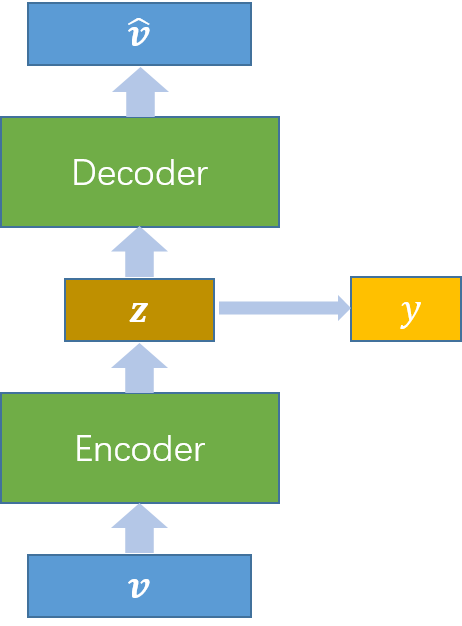
\includegraphics[width=0.5\textwidth]{label_vae.png}
  \caption{结合label预测的VAE模型}
  \label{fig:label_vae}
  %\vspace*{-0.6em}
\end{figure}
受~\autocite{Kingma2014Semi}的启发,HAVAE引入了标签信息。如图~\ref{fig:label_vae},在图~\ref{fig:vae}的基础上加入了对标签的预测,图中右侧的$\bm y$表示在$\bm z$的基础上预测的标签向量,在有可用标签的任务中,加入标签信息可以提高模型的学习效果。所以,HAVAE的损失函数包括两部分——VAE损失函数和标签损失函数,即
\begin{equation}
\label{eq:loss}
\mathcal L= \mathcal L_{vae}+\alpha\mathcal L_{label}.
\end{equation}
\par


\subsubsection{VAE的损失函数}
模型最终学习到的歌词的表征向量为$\bm{\mu_z}$,即$\bm{v_t} = \bm{\mu_z}$。VAE的损失函数$\mathcal L_{vae}$如下所示:
\begin{equation}
    \mathcal{L}_{vae}=-D_{\mathcal{KL}}(\mathcal{Q}(\bm z|\bm v)||\mathcal{P}(\bm z))+\log\mathcal{P}(\bm v|\bm z),
\end{equation}
其中,$-D_{\mathcal{KL}}(\mathcal{Q}(\bm z|\bm v)||\mathcal{P}(\bm z))$是生成损失,$-\log\mathcal{P}(\bm v|\bm z)$是重构损失。\par

令$ \mathcal Q( \bm z|\bm v)$为$ \bm z $的近似先验分布,$ P\left(\bm z\right) $为$ \bm z $的先验分布。VAE模型的目标是最小化$\mathcal Q (\bm z|\bm{v})$和$\mathcal P\left(\bm z\right) $之间的差距。此处引入了$\mathcal{KL}$散度(Kullback-Leibler divergence):
\begin{equation}
    D_{\mathcal{KL}}(\mathcal{Q}(\bm z|\bm v)||\mathcal{P}(\bm z))=\sum _{i=1}^{N}\mathcal{Q}(\bm {z_i}|\bm {v_i}) \times \log { [{\mathcal{Q}(\bm {z_i}|\bm {v_i})}/{\mathcal P\left(\bm z_i\right)}]}.
\end{equation}
因为先验分布和后验分布都是高斯分布,等式可以被简化为:
\begin{equation}
    D_{\mathcal{KL}}(\mathcal{Q}(\bm z|\bm v)||\mathcal{P}(\bm z))=\frac{1}{2}\sum_{i=1}^{N}(1+\log(\bm{\sigma_z})_i^2-(\bm{\mu_z})_i^2-(\bm{\sigma_z})_i^2).
\end{equation}
\par

重构损失部分可以理解为最大化从隐含向量$\bm z$重构出输入向量$\bm v$的概率。由于解码部分是一个多元高斯分布,所以这里本文采用了对数损失函数,因此重构损失为:
\begin{equation}
    -\log\mathcal{P}(\bm v|\bm z)=-log\mathcal{N}(\bm v; \bm{\mu_{\hat{v}}}, \bm{\sigma_{\hat{v}}^2I}).
\end{equation}
\par

\subsubsection{标签损失函数}
本文引入了一个标签向量$\bm y$。$\bm y$的维度等于所有样本的类别总数。在HAVAE中,由$\bm v_t$通过$\bm {\hat{y}} = F(\bm{\mu_z})$计算得出对歌词标签的估计$\bm {\hat{y}}$,其中$F$是一个带‘sigmoid’激活函数的全连接层。标签损失函数是$\bm {\hat y}$和歌词真实标签$\bm y$之间的差距,本文中标签损失函数为$\bm {\hat y}$和$\bm y$的交叉熵,即:
\begin{equation}
  \mathcal{L}_{label}=-\frac{1}{N}{\sum_{i=1}^N}\frac{1}{M}{\sum_{j=1}^{M}}(y_{i,j}{\log {Y}_{i,j} }+(1-Y_{i,j})\log(1-y_{i,j})),
\end{equation}
其中$M$是标签集合的大小,即$\bm y$的维度。
\par

\section{本章小结}
本章首先介绍了HAVAE模型的特征提取模块。对于韵律特征,本文主要关注与英美韵律文学中常见的两种韵律——单韵模式和隔行韵模式。韵律特征的提取应用到了rhyme2vec模型。rhyme2vec分别先获取了一段韵律文本中与这两种韵律模式相对应的韵律段($\bm {L_r^m}$、$\bm {L_r^o}$和$\bm {L_r^e}$)的音素符号,然后从这几个韵律段中学习到了相应的韵律向量,再应用注意力机制将这几个韵律段结合到一起,得到整段文本的韵律表征向量$\bm {v_r}$。对于语义特征的提取,本文采用了目前效果较好的文本表征学习模型doc2vec。\par

之后本章介绍了HAVAE模型的特征融合模块。特征融合模块是一个结合层次注意力机制的VAE模型。特征融合模块的输入为特征提取模块输出的韵律表征向量$\bm {v_r}$和语义表征向量$\bm{v_s}$。$\bm {v_r}$和$\bm{v_s}$在特征融合模块中首先通过注意力机制结合到一起,得到一个整体的表征向量$\bm {v}$,之后输入到一个VAE模型中,经过一个编码过程和解码过程,重构出一个向量$\bm {\hat v}$,通过最小化$\bm {v}$和$\bm {\hat v}$之间的差距来优化,最终得到编码出的向量$\bm{v_t}$作为整段文本的表征向量。\par

\chapter{实验设计与结果分析} \label{chpt:exp}

\section{数据集与实验设计}
考虑到在线的韵律文本资源很少,本文采用了从网上爬取的一个说唱歌词语料库~\footnote{http://ohhla.com/}。这个语料库包括3154名歌手的65730首歌。\par

\begin{sloppypar}
为进行数据清洗,根据~\autocite{Malmi2016dopelearning},所有标题包含“intro”、“outro”、“skit”、“interlude”和“remi”的歌曲都被从数据集中剔除。在大多数的说唱歌曲中,常见的部分包括包括序曲、副歌、主歌和结尾。在这些部分中,主歌占据主要地位~\footnote{https://rappingmanual.com/lesson-rapping-song-structure-learn-how-to-rap/},所以本文的数据集只保留了主歌部分。\par
\end{sloppypar}

\section{NextLine预测} \label{sec:nextline}
NextLine预测任务由~\autocite{Malmi2016dopelearning}提出的。给定一首$n$行的说唱歌曲,假设其前$k~(k<n)$行(记作$\bm Q=\{s_1,s_2,...,s_k\}$)已知。令$\bm C={\left\{c_1,c_2,...,c_m\right\}}$表示$m$行候选歌词。此任务的目的就是从$\bm C $中找到歌词的第$k+1$行,即$s_{k+1}$;换句话说,与$s_{k+1}$最相关的歌词$c_i~(1\leq i \leq m)$将被选作匹配目标。\par

\subsection{数据集} \label{subsec:nextdata}
在此实验中,数据集中的所有说唱歌词都被分成单行的歌词,最终从16697首歌词中分出810567行单独的歌词。整个数据集分为训练集(50\%)、测试集(25\%)和验证集(25\%)。\par

\subsection{对比方法} \label{sec:nextlinebaseline}
本文选择了以下几种方法作为对比方法:
\begin{itemize}
  \item{\bf EndRhyme}~\autocite{Malmi2016dopelearning},该方法通过计算候选歌词行$l_i$和$s_k$结尾匹配元音音素的个数来寻找最适合的下一行;
  \item{\bf rhyme2vec},该方法即为~\ref{chpt:model}\ref{sec:fe}中所描述的韵律表征学习方法;
  \item{\bf NN5}~\autocite{Malmi2016dopelearning},该方法是一个字符级别的神经网络。该神经网络将每首歌的最后5行作为查询对象,并将其编码后,寻找最合适的下一行;
  \item{\bf doc2vec}~\autocite{quoc2014distributed},该方法为当前最好的文本段落表征学习方法之一,在这个方法中将$\{s_k;l_i\}$作为一个段落;
  \item{\bf DopeLearning}~\autocite{Malmi2016dopelearning}~\footnote{本文中只采用了其最原始的方法,并进行了复现。由于NN5方法没有提供源代码,且其结果并没有明显提升,本文中并没有将其加入DopeLearning方法中。},该方法是目前最好的说唱歌词表征学习方法。它将一系列的统计特征组合到一起,包括EndRhyme、EndRhyme-1~\footnote{不同于EndRhyme,EndRhyme-1统计的是$c_i$和$s_{k-1}$结尾匹配的元音音素的个数。}、OtherRhyme~\footnote{OtherRhyme统计的是每个单词中匹配元音音素个数的平均数。}、LineLength~\footnote{LineLength从句子长度的角度计算$c_i$和$s_k$的相似度。}、BOW~\footnote{BOW利用Jaccard距离以及词袋模型计算$s_k$和歌曲最后5行的相似度。}、LSA~\footnote{计算$c_i$和$s_k$之间的LSA相似度。}以及NN5~\footnote{NN5模型最后$softmax$层的置信度值。};
  \item{\bf early fusion}~\autocite{Malmi2016dopelearning, chen2017visual},该方法在多模态融合问题中很常见,所有输入向量都将被拼接在一起作为一个统一的表征向量,即$\bm {v_t}=[\bm{v_r};\bm{v_s}]$;
  \item{\bf EF-AE},该方法将$[\bm{v_r};\bm{v_s}]$输入一个自编码器(autoencoder,以下简称AE)网络得到最终的表征向量;
  \item{\bf EF-VAE},该方法将$[\bm{v_r};\bm{v_s}]$输入一个VAE网络得到最终的表征向量。
\end{itemize}
根据利用到的输入信息,这些方法可以被分为三类,即韵律类、语义类和结合类(结合了韵律和语义信息)。\par

\subsection{实验设置}
在训练阶段,采用了负采样的方法,即每一个查询行$s_m$都有两个候选歌词行,其中一行是该歌词真正的下一行,作为正例;另一行是从语料库中的其他歌词中随机选择的一行,作为反例。在测试阶段,每一个查询都有一个300行的候选集,其中包含真正的下一行以及299个随机选择的歌词行。\par

实验将每一个查询与其每一行候选歌词分别结合为一对作为输入。与BOW5和NN5不同~\footnote{这两种方法在提取语义特征时考虑了查询歌词的最后五行。},本实验中只考虑了查询歌词的最后一行$s_m$。$\alpha$的值设为1。$\bm{v_r}$和$\bm{v_s}$的维度设为125。根据~\autocite{Malmi2016dopelearning},DopeLearning得到的表征向量最终被输入到SVM$^{rank}$~\autocite{thorsten2006training}工具进行排名。而其他方法得到的表征向量维度都较高,并不适用SVM$^{rank}$。本实验设计了一个排名层用于计算每对数据的分数,计算方式为$score=sigmoid(W\bm{v_t}+b)$,其中$score~(0-1)$是候选歌词行和查询行之间的相关性,$score$越高越好。模型网络中全连接层的激活函数均选用了$tanh$。模型的优化器选用了$Adadelta$~\autocite{zeiler2012adadelta}。模型的训练轮数为20。\par

\begin{table}[h]
  \centering
  \caption{本文模型与对照方法的结果对比}
  %\vspace*{-1em}
  \scalebox{0.65}{
  \renewcommand{\arraystretch}{1.3}
    \begin{tabular}{p{6em}p{8em}cccccc}
      \toprule
      \multicolumn{1}{l}{信息} & 方法 & mean rank & MRR   & Rec@1 & Rec@5 & Rec@30 & Rec@150 \\
      \midrule
      \multicolumn{1}{l}{\multirow{2}[0]{*}{韵律特征}} & EndRhyme & 103.2* & 0.140* & 0.077* & 0.181* & 0.344* & 0.480* \\
      \cmidrule{2-8}
      & rhyme2vec &17.7&0.463&0.347&0.592 &0.841&0.981  \\      
      \midrule
      \multicolumn{1}{l}{\multirow{2}[0]{*}{语义特征}} & NN5& 84.7* & 0.067* & 0.020* & 0.083* & 0.319* & 0.793* \\
      \cmidrule{2-8}
      & doc2vec &15.5&0.430&0.293&0.588&0.870&0.985\\
      \midrule
      \multirow{6}[0]{*}{融合特征} & DopeLearning & 60.8*/79.9 & 0.243*/0.168 & 0.169*/0.102 & 0.304*/0.220 & 0.527*/0.446 & 0.855*/0.775 \\
      \cmidrule{2-8}
      & early fusion &9.6&0.588&0.464&0.738&0.926&0.991\\
      \cmidrule{2-8}
      & EF-AE &5.3&0.771&0.683&0.879&0.966&0.995\\
      \cmidrule{2-8}
      & EF-VAE &2.3&0.941&0.914&0.973&0.990&0.997\\
      \cmidrule{2-8}
      & \textbf{HAVAE} &\textbf{1.2}&\textbf{0.982}&\textbf{0.973}&\textbf{0.993}&\textbf{0.999}&\textbf{1.000}\\     
      \midrule
      \multicolumn{8}{l}{\small 带*的结果是~\autocite{Malmi2016dopelearning}中展示的结果,其他结果都是根据本文中设置重新运行得到的结果。} \\
      \bottomrule
    \end{tabular}%
    \renewcommand{\arraystretch}{2}
  }
  \label{table:results}%
\end{table}%

\subsection{结果评估与分析} \label{subsec:nextresult}
实验结果由mean rank、mean reciprocal rank(以下简称MRR)和Rec@n($n=1,5,30,150$)三个标准评估进行评估。令$Q$表示查询行序列,$r_i$表示在第$i$个查询中正确的下一行在候选歌词中的排名。mean rank是$r_i$的平均值,范围在$[1, 300]$,越小越好。MRR是$\frac{1}{r_i}$的平均值,越大越好。Rec@n是${r_i} {\leq} n$的频率,值越大越好。\par

实验结果如表~\ref{table:results}所示。显然,本文提出的方法比其他对比方法的性能都要突出,达到了目前最高的水平。从结果中,主要有如下发现:

\subsubsection{HAVAE的有效性}在所有的这些方法中,本文提出的模型取得了最好的效果。mean rank值为\textbf{1.2},极为接近1,远优于其余方法中最好的方法。DopeLearning的原始论文中,mean rank为60.8,而本文复现的结果为79.9,二者皆高于60。在MRR方面,本文模型的方法结果为0.982,优于DopeLearning的0.168和0.243。在Rec@n上的性能展示了相似的情况——本文模型得到了远好于其他方法的结果。总的来说,本文的模型比当前最好的方法表现更好,表明本文提出的模型是有效的。造成这种差距的主要原因是提取了更有效的韵律特征和语义特征(分布式表征学习而非简单的统计学特征),并进行了适当的融合(基于VAE的框架)。\par

\subsubsection{rhyme2vec的有效性}与EndRhyme相比,rhyme2vec很明显在实验中的几个评价标准(mean rank、MRR和Rec@k)上都得到了比其他方法更好的结果。这种结果表示本文提出的方法rhyme2vec学习到的韵律表征向量,通过考虑多种韵律模式,得到了比其他方法得到的韵律向量更为有效。\par

\subsubsection{韵律信息对整体表征向量的提升}由表格中数据可见,单独利用语义表征(doc2vec)或韵律表征(rhyme2vec)的结果都较差(mean rank大于15,MRR小于0.5)。而将两种特征融合后,最终结果得到了显著提升。同样的情况在DopeLearning中也得到了体现,DopeLearning的结果也要好于单独应用EndRhyme或NN5特征。这两个结果同时证明了同时利用韵律特征和语义特征可以得到更好的效果。\par

\subsubsection{特征融合模型的有效性}early fusion方法将所有特征的表征向量进行拼接,得到的向量作为最终的融合向量(与DopeLearning相同的方法),最终在mean rank和MRR上分别得到了9.6和0.588的结果。与early fusion相比,可以看到EF-AE得到了更好的结果,其原因有可能是因为EF-AE加入了自编码器网络,学到了不同特征之间的相互联系~\autocite{bengio2009learning}。另外,EF-VAE的表现比EF-AE更好,这也表明VAE在这个歌词学习的任务上比AE模型更为有效。而HAVAE模型比EF-VAE的结果更好,表明注意力机制的有效性,其结果的提升是因为注意力机制强化了语义和韵律信息之间的练习,提升了模型的效果。\par

\subsubsection{其他发现} \label{sssec:other}实验结果显示,doc2vec在mean rank上的结果优于rhyme2vec。相似的,NN5网络的结果在mean rank上同样优于EndRhyme。这有可能是由于在歌词中,语义信息比韵律信息更为重要。然而从MRR和Rec@n的结果来看,rhyme2vec在MRR、Rec@1、Rec@5上的结果比doc2vec更好,这说明 rhyme2vec 得到的结果更为极端doc2vec,即预测的结果中给更多的正确结果预测了一个很高或很低排名,而doc2vec则会得到一个更为中庸的结果,给更多的正确结果预测到了一个中上的位置。\par

\begin{table}[h]
  \caption{不同韵律模式的性能}
  \centering
    \scalebox{0.95}{
    \renewcommand{\arraystretch}{1.3}
    \begin{tabular}{ccc}
      \toprule  
      \rule{0pt}{12pt}    
      \textbf{韵律模式}& \textbf{mean rank} & \textbf{MRR} \\[2pt]\midrule
      \rule{0pt}{12pt}
       \textbf{C-Line} & 60.1030  & 0.1542 \\
       \textbf{Skip-Line} & 61.3070  &   0.1498\\
             \textbf{sum} & 24.0840  &   0.4067\\
       \textbf{rhyme2vec}  &\textbf{17.0810} & \textbf{0.4714} \\
      [1pt]
            \bottomrule    
    \end{tabular}}
    \renewcommand{\arraystretch}{1}
  \label{table:rs}
\end{table}

为探索不同韵律模式对结果的贡献,本文还分别对C-Line韵律向量、Skip-Line韵律向量和两种向量的和向量sum进行了实验,实验结果如表~\ref{table:rs}所示。由结果可知,C-Line的结果略微好于Skip-Line,但差距并不明显,说明在说唱歌词中,单韵模式和隔行韵模式的重要性基本相同;而sum的结果优于C-Line和Skip-Line说明同时学习单韵模式和隔行韵模式可以明显提升模型的性能,两种韵律模式的结合是有价值的;rhyme2vec的结果好于sum,也再一次证明了注意力机制的有效性。\par

\subsection{参数讨论}
为优化模型效果,本文还对模型进行了参数讨论,包括公式~\ref{eq:loss}中的$\alpha$、语义特征模块输入行数$k$以及模型在每轮的实验结果和损失函数。\par

\begin{figure}[h]
    \centering
    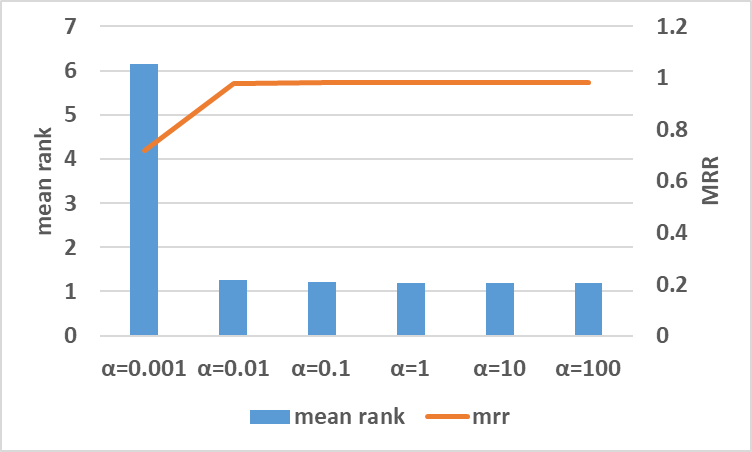
\includegraphics[width=12cm]{alpha.png}
    \caption{$\alpha$对结果的影响}
    \label{fig:alpha}
\end{figure}
对参数$\alpha$的讨论结果如图~\ref{fig:alpha}所示,实验只是对$\alpha$的数量级进行了讨论,这是因为,在同一数量级,$\alpha$对于实验结果的影响并不明显。$\alpha$的数量级从$0.01$到$1$时,效果有所提升,其中从$0.01$到$0.1$的提升最为明显;当$\alpha = 1$时,模型的效果达到了最高值,mean rank约为$1.3$,MRR约为$0.977$;$\alpha$的数量级从$1$到$100$时,模型的效果逐渐变差。这表明加入标签信息对于模型的训练有所提升,且当模型在训练时对,标签损失和VAE损失的权重相同时模型的效果更好,更说明了标签信息的有效性。\par

\begin{figure}[h]
    \centering
    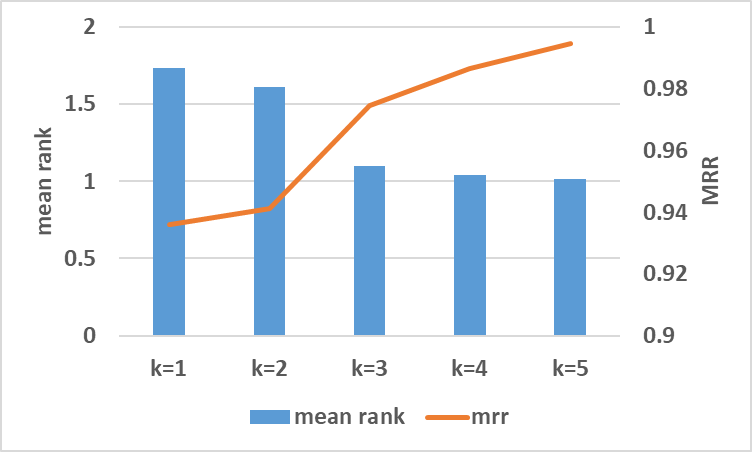
\includegraphics[width=12cm]{k.png}
    \caption{$i$对结果的影响}
    \label{fig:k}
\end{figure}
对参数$i$的讨论结果如图~\ref{fig:k}所示,这里为了更明显地体现$i$的影响,没有用HAVAE模型进行参数讨论,而是单纯用语义特征提取模块doc2vec模型进行了参数讨论。从图中可见,随着$i$的提升,实验效果明显提升,说明更多的查询行更有利于NextLine预测的实验效果。但是由于提高$k$的时间开销太大,所以最终实验时只选取了$i=1$。\par

\begin{figure}[h]
    \centering
    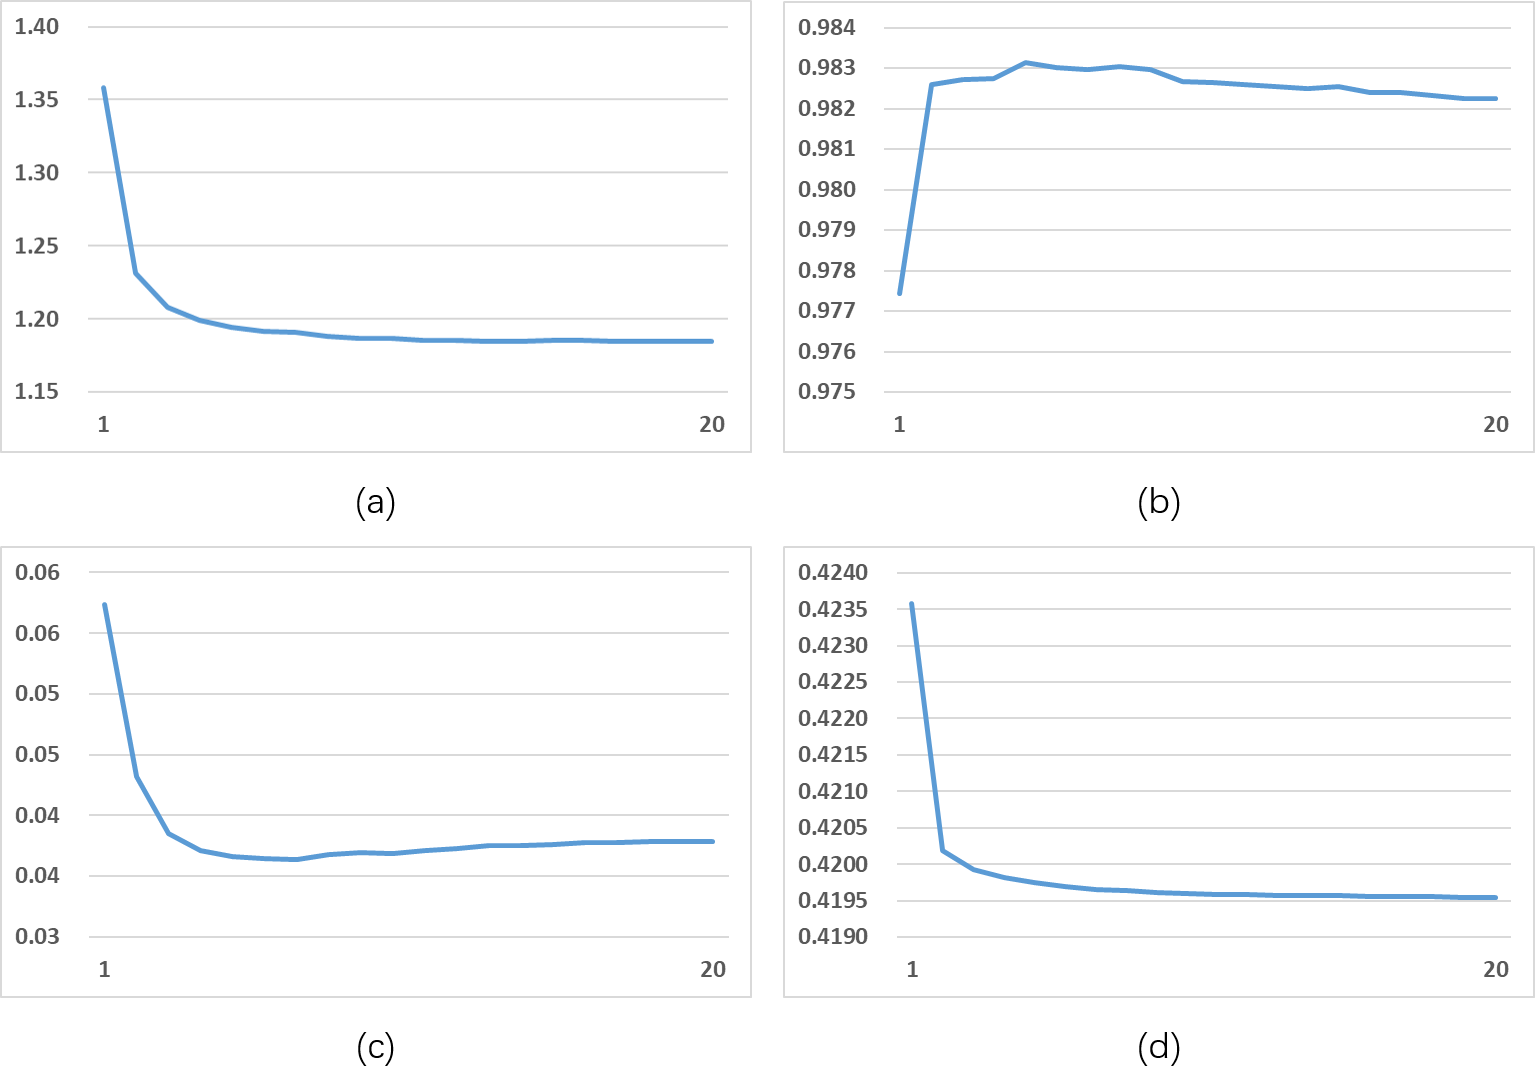
\includegraphics[width=14cm]{epoch.png}
    \caption{模型评价结果和损失函数随训练过程的变化}
    \label{fig:epoch}
\end{figure}

本文还对模型训练过程中mean rank分数、MRR分数和损失函数的变化进行了记录,结果如图~\ref{fig:epoch}所示,(a)为模型的mean rank得分,(b)为模型的MRR得分,(c)为模型的标签损失函数$\mathcal L_{label}$,(d)为模型的VAE损失函数$\mathcal L_{vae}$,每幅图的横轴为模型训练的轮数。由图~\ref{fig:epoch}(a)可知,模型在训练到第3-4轮时,mean rank分数就已达到1.2以下;由图~\ref{fig:epoch}(b)可知,模型在训练到第四轮时,MRR分数达到了最高值;由图~\ref{fig:epoch}(c)可知,模型在训练到第4-5轮时,$\mathcal L_{label}$达到了最低值;由图~\ref{fig:epoch}(d)可知,模型的$\mathcal L_{vae}$虽然一直在下降,但在第3-4轮后便趋于平稳。由以上发现可知模型收敛速度很快,分析有可能是由于数据量太小导致的。\par

\section{说唱歌曲生成}
基于NextLine预测实验,本文进行了另一个实验,即说唱歌词生成。该实验给定一系列单行的说唱歌词$\bm L = \{l_1, l_2, ... , l_n\}$,以及一个候选歌词集合$\bm C = {c_1, c_2, ..., c_m}$,其中,$n$为集合$\bm L$的大小,$m$为集合$\bm C$的大小。对于$\bm L$中的每行歌词$l_i~(1 \leq i \leq n)$,模型需要从$l_i$出发,利用候选歌词生成一段$t$行的说唱歌词。实验的对比方法选择了DopeLearning~\autocite{Malmi2016dopelearning}。\par

\subsection{数据集}
实验所用的$\bm L$是从~\ref{subsec:nextdata}所述数据集中随机挑选的100行歌词,$\bm C$中包含810567行歌词。\par

\subsection{实验设置}
令$T_{i,j}$为从$l_i$出发,生成的$j$行的歌词段。模型要从初始歌词$l_i$(亦即$T_{i, 1}$)开始,生成一段$t$行的歌词,需要经过$t-1$次预测,第$j$次预测的输入为$T_{i, j}$,模型得到输入后,将从$\bm C{}$中挑选出最有可能的下一行歌词$c$,将$c$接在$T_{i, j}$的末尾,得到$j+1$行的歌词段$T_{i, j+1}$作为第$j+1$次预测的输入。为避免生成歌曲中出现重复歌词,实验中每一步都会将所选作为下一行的歌词从$\bm C$中剔除。本文将最终生成歌词的长度$t$设置为$16$。实验中的模型均为通过~\ref{subsec:nextdata}所述下一行实验的数据集训练得到的模型。\par

\subsection{结果评估及分析}
\subsubsection{评价标准}
好的说唱歌词的应该通顺、流畅,主题应该明确,并且韵律应该足够有吸引力。然而,歌词的流畅度、主题的明确程度并没有一个量化的评价方法,而完全靠人工评估并不客观,且需要大量的人力与经济成本。因此,本文只采用了对韵律的量化评价方法来评价模型生成的说唱歌曲。\par

本文采用了两种韵律密度评分,称为RD2010和RD2016。RD2010由~\autocite{hirjee2010using}提出,该评价标准将一首歌词中押韵的音节在所有音节中所占比例作为对该首歌词的韵律密度评分,一首歌词的RD2010分数越高,说明该歌词押韵的语句越多。RD2016由~\autocite{Malmi2016dopelearning}提出,该评价标准通过计算一首歌词中相邻行单词的最长匹配元音序列的平均值来计算该首歌词的韵律密度分数,一首歌词的RD2016分数越高,说明该首歌词相邻行单词之间押韵越多。\par

\begin{figure}[h]
    \centering
    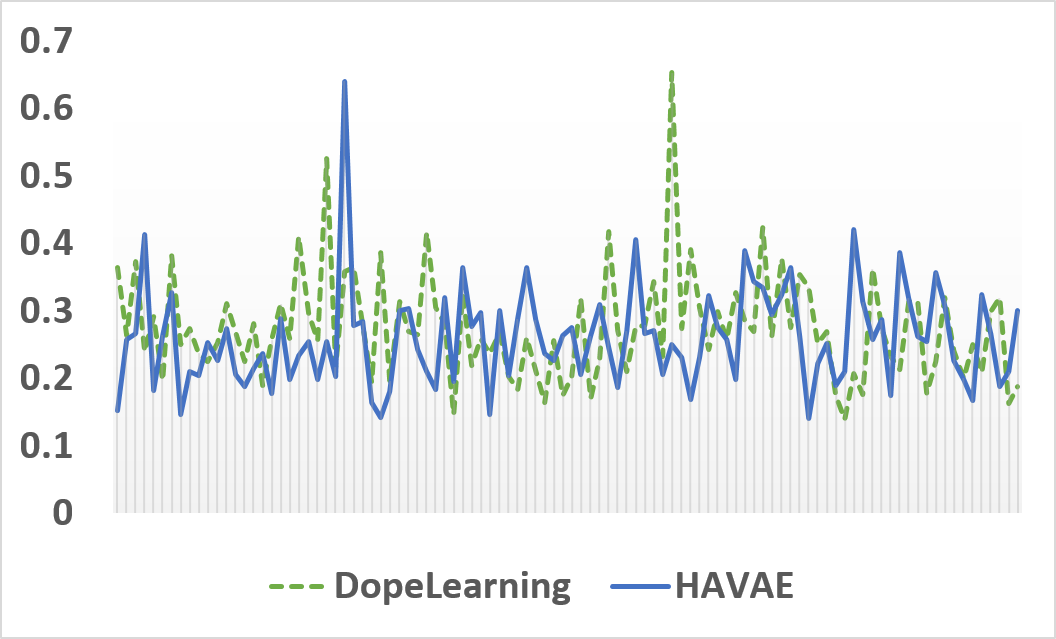
\includegraphics[width=12cm]{rd2010.png}
    \caption{RD2010分数}
    \label{fig:rd2010}
\end{figure}
\begin{figure}[!h]
    \centering
    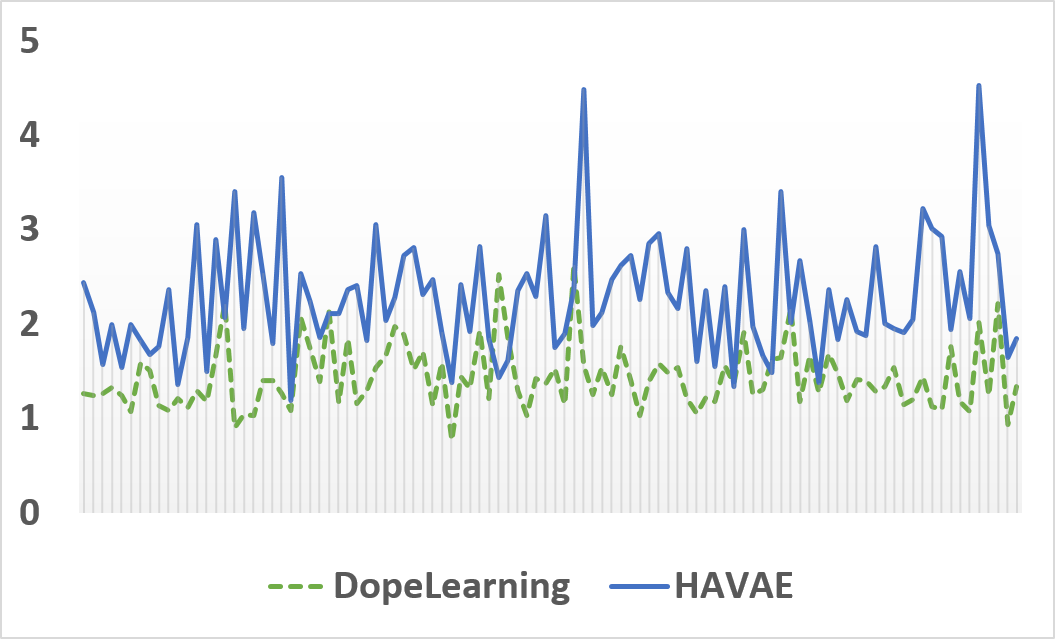
\includegraphics[width=12cm]{rd2016.png}
    \caption{RD2016分数}
    \label{fig:rd2016}
\end{figure}

\subsection{实验结果分析}

实验结果如图~\ref{fig:rd2010}和图~\ref{fig:rd2016}所示。由图~\ref{fig:rd2010}和图~\ref{fig:rd2016}可见,HAVAE和DopeLearning在RD2010上的整体得分情况比较接近;而在RD2016上,HAVAE的得分明显高于DopeLearning,仅在个别歌曲中,HAVAE的得分低于DopeLearning。由以上结果可知,HAVAE所生成歌词的韵律比DopeLearning所生成歌词更好,同~\ref{subsec:nextresult}得到了相同的结论。\par

\section{说唱歌词流派分类} \label{sec:clf}
为展示HAVAE和rhyme2vec的泛化能力,本文设计了歌曲级别的说唱流派多标签分类任务作为补充。给定一个说唱歌曲的集合$\bm S = \{s_1, s_2, ... , s_N\}$和一个说唱歌词的标签集合$\bm G = \{g_1, g_2, ... , g_M\}$,要求预测出每一首歌的标签集合,即每首歌对应多个标签,其中$N$是集合$\bm S$的大小,$M$是集合$\bm G$的大小。也就是说,该任务是一个多标签分类任务。\par

\subsection{数据集}
本文采用了一个包含10167首歌曲和9种流派\footnote{这9种流派包括Alternate、Christian、East Coast、Grime、Hardcore、Horrorcore、Midwest、Southern和West Coast。}的流派分类数据集,即$\bm G$的大小$M=9$,数据集中$9$种标签的数量如表~\ref{table:genre}所示。数据集中每首歌词都对应一名歌手,歌手则对应了一个标签集合$\bm {G_i}$,该首歌词的标签集合即为该名歌手对应的标签集合。数据集分为训练集和测试集,训练集包含9150首歌曲,测试集包含1017首歌曲。\par

\begin{table}[h]
\centering
\caption{数据集中流派标签数量分布}
\label{table:genre}
\begin{tabular}{ccccccccc}
\toprule
0   & 1   & 2    & 3   & 4    & 5   & 6    & 7    & 8    \\ \midrule
638 & 336 & 3507 & 268 & 1178 & 793 & 1192 & 3680 & 2375 \\ \bottomrule
\end{tabular}
\end{table}

\subsection{对比方法}
\begin{itemize}
  \item{\bf RhymeAPP}~\autocite{hirjee2010rhyme},该方法是一个计算说唱歌词统计特征的歌词分析工具;
  \item{\bf rhyme2vec},该方法即为~\ref{chpt:model}\ref{sec:fe}中所描述的韵律表征学习方法;
  \item{\bf doc2vec}~\autocite{quoc2014distributed},该方法同~\ref{sec:nextlinebaseline},将整首歌词作为一个段落进行学习;
  \item{\bf HAN-L}~\autocite{Tsaptsinos2017lyrics},该方法是当前最优秀的歌词流派分类方法,采用了循环神经网络(recurrent neural network,即RNN),并在词和句子层面分别应用了注意力机制,该方法仅学习了语义特征。
\end{itemize}

\subsection{实验设置}
本实验将歌词输入到各个模型中,得到相应的特征向量,然后将这些特征向量输入一个分类网络中,该网络为每一个输入样本计算出一个$9$维的向量$\bm y$,$\bm y$的每一个元素对应一个流派,表示一首歌属于该流派的可能性。该分类网络有一个参数,即阈值$t$,用于决定一首歌是否属于某个流派,此过程如下所示:
\begin{equation}
    \bm {y'_i}=\left\{
    \begin{aligned}
    0 , \quad if \ \bm{y_i}\leq t\\
    1 , \quad if \ \bm{y_i}> t\\
    \end{aligned}
    \right.
\end{equation}
最终$\bm {y'_i}$为分类结果。\par

\subsection{结果评估及分析}
\begin{figure}[!h]
    \centering
    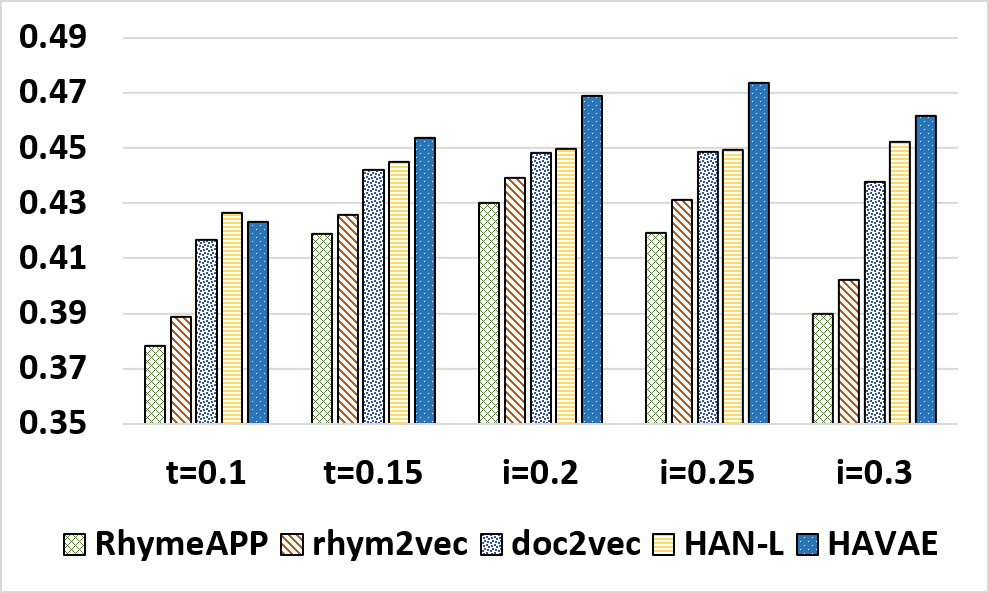
\includegraphics[width=12cm]{micro.png}
    \caption{micro-f1分数}
    \label{fig:micro}
\end{figure}
\begin{figure}[!h]
    \centering
    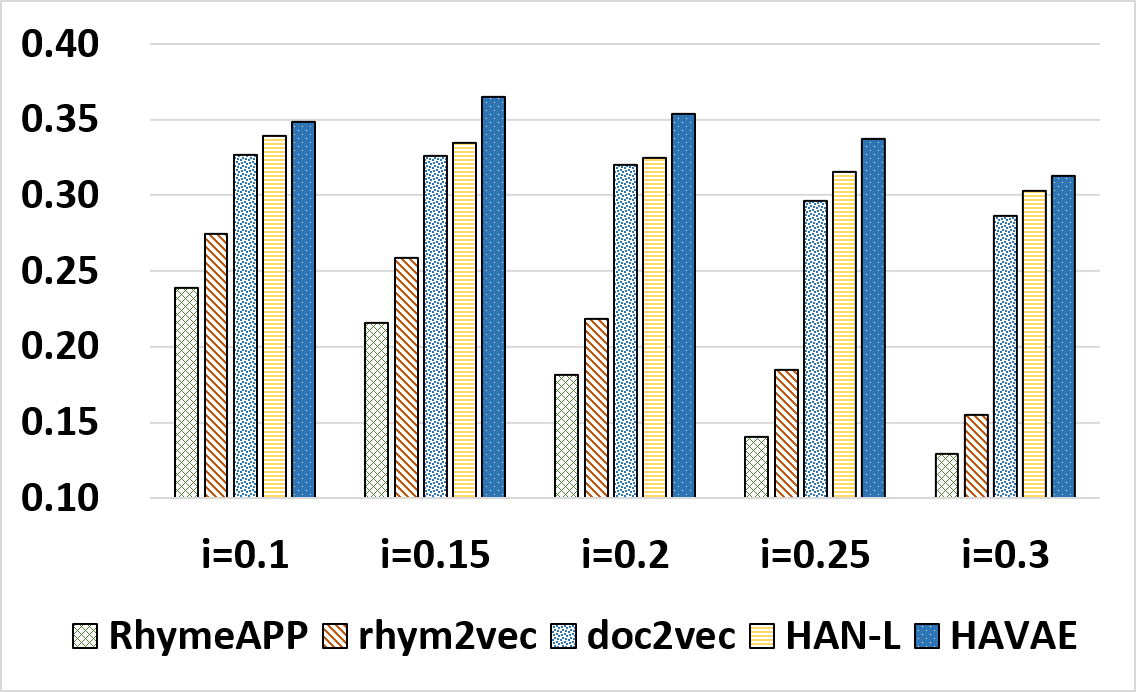
\includegraphics[width=12cm]{macro.png}
    \caption{macro-f1分数}
    \label{fig:macro}
\end{figure}
本文用micro-f1和macro-f1两个标准来评估最终的分类结果。f1是一种用来结合precision和recall评估结果的评价标准,micro-f1和macro-f1是对f1不同的平均方式。\par
micro-f1的计算方式如下:
\begin{equation}
  \label{eq:micro}
  \begin{gathered}
    precision_{micro} = \frac{\sum^m_{i=1}TP_i}{\sum^m_{i=1}(TP_i + FP_i)}\\
    recall_{micro} = \frac{\sum^m_{i=1}TP_i}{\sum^m_{i=1}(TP_i + FN_i)}\\
    micro-f1 = \frac{(\beta^2 + 1) \times precision_{micro} \times recall_{micro}}{\beta^2 \times precision_{micro} + recall_{micro}}
  \end{gathered}
\end{equation}
其中$TP_i$为第$i$类中true positive的数量,$FP_i$为第$i$类中的false positive的数量,$FN_i$为第$i$类中的false negative的数量。\par
macro-f1的计算方式为:
\begin{equation}
  \begin{gathered}
    precision_i = \frac{TP_i}{TP_i + FP_i}\\
    recall_i = \frac{TP_i}{TP_i + FN_i}\\
    f1_i = \frac{(\beta^2 + 1) \times precision_{i} \times recall_{i}}{\beta^2 \times precision_{i} + recall_{i}}\\
    micro-f1 = \frac{\sum_{i=1}^mf1_i}{m}
  \end{gathered}
\end{equation}
其中$TP_i$、$FP_i$和$FN_i$的含义与公式~\ref{eq:micro}中相同。\par

最终的分类评估结果如图~\ref{fig:micro}和图~\ref{fig:macro}所示。总的来说,在大部分情况下,HAVAE比其他方法的效果更好,尤其是当$t=0.2$的时候。从结果中,主要有以下发现:
\subsubsection{HAVAE在歌曲级别的有效性} 与NextLine预测任务不同,歌词流派分类任务的数据是在歌曲级别上。而从图~\ref{fig:micro}和图~\ref{fig:macro}中可以看到,HAVAE仍然比其他方法更为有效。由此可见,输入数据中单个样本的长短并不会对HAVAE的效果造成很大影响,此结果可以在一定程度上说明HAVAE的泛化能力较好。\par

\subsubsection{语义与韵律特征的重要性} 由表~\ref{table:results}和~\ref{sssec:other}可知,在NextLine预测任务中,doc2vec和rhyme2vec的结果相差并不多,然而,在歌词流派分类中,doc2vec的结果却远优于rhyme2vec的结果,出现这种结果,很有可能是因为,对于歌词中的几行,韵律的模式更为明显,很有可能只有一种韵律模式;而对于整首歌词,可能会有多种韵律模式的混合,韵律特征的效果会受到一定的影响。而语义特征并不会受到这种影响,反而有可能因为短文本中包含的语义不完整而导致整首歌词的学习效果相对于部分歌词的学习效果有所提升。当然,不排除doc2vec模型比rhyme2vec模型更适用于多标签分类任务。\par

\section{本章小结}
本章通过三个实验从不同的角度证明了HAVAE模型的有效性。\par
首先是NextLine预测实验,这个实验给定一组文本段作为查询集,一组文本行作为候选集,实验的模型要根据每一个查询段进行检索,将候选行按出现在查询段下一行的可能性排序,最有可能出现在下一行的排在最前。最终,在mean rank评价标准上,HAVAE模型比表现最好的对比方法DopeLearning的效果高出一个数量级;在MRR评价标准上,HAVAE比DopeLearning的效果高3倍。另外,实验还通过分别测试不同韵律模式模型和rhyme2vec模型,证明了rhyme2vec模型中注意力机制的有效性。\par

之后是歌曲生成实验,该实验建立在在NextLine预测实验的基础上。实验的输入为一组单行的歌词,以及一个候选单行歌词集。模型需要以每一个输入的单行歌词为现有文本,从候选的单行歌词集中重复的挑选下一行,与现有文本组成新的输入,直到生成所需长度的歌词。实验的评价标准为RD2010和RD2016。在RD2010上,HAVAE的效果和对比方法DopeLearning的表现接近,而在RD2016上,HAVAE的效果则明显高于DopeLearning。NextLine预测实验和歌曲生成实验证明了HAVAE模型在韵律文本检索任务上的有效性。\par

最后,本章介绍了歌词流派分类实验。该实验的数据包括一个歌词集合,以及集合中每首歌词对应的流派标签。模型通过分析每一首歌词,对其进行流派分类。最终,在macro-F1和micro-F1两个评价标准上,HAVAE都明显高于其他对比方法。该实验证明了HAVAE模型在韵律文本分类任务上的有效性。\par

\chapter{结论与展望} \label{chpt:conclusion}
韵律文本是一种特殊类型的文本,相对于通俗的自然语言,韵律文本分析与学习值得进行专门的研究。然而目前韵律文本分析与学习存在以下一些问题:韵律文本分析与学习的数据是非结构化的,相对于结构化数据,非结构化数据中难以获取计算机需要的形式语义,因此通过计算机进行处理和分析有很大难度;且相对于自然语言,韵律文本中还添加了韵律和形式的特征,而现有的NLP技术由于没有考虑韵律和结构的特征,并不适合直接应用于韵律的分析;不同类型的韵律文本的结构和韵律特征差异较大,一种算法难以广泛应用于大部分的韵律文本学习任务;许多韵律文本学习方法并没有充分利用韵律文本的特征,许多都只是单纯利用了韵律文本的语义特征或韵律特征,没有把二者结合分析;许多韵律文本学习方法是针对特定类型的韵律文本进行的,泛用性很差。\par

为解决以上问题,本文提出了rhyme2vec和HAVAE两个模型。rhyme2vec用来学习韵律表征向量。这个方法包含两个模型,即连续行韵律和隔行韵律。通过整合这两个模型,rhyme2vec可以很好地处理韵律模式的多种特征。HAVAE用于融合韵律文本的韵律特征和语义特征。该框架旨在处理韵律文本的表征学习问题,利用注意力机制对韵律信息进行了有效整合且对语义与韵律信息进行了无缝整合。\par

最终,本文通过实验验证了rhyme2vec和HAVAE训练得到的表征向量在检索和分类等任务上的有效性,实验包括NextLine预测、流派分类、歌词生成。通过与现有的一些表现较好的韵律文本学习方法进行比较,最终结果显示rhyme2vec和HAVAE相对于这些方法更为有效。在NextLine预测实验中,HAVAE模型在 mean rank评价标准上比表现最好的对比方法DopeLearning的效果高出一个数量级;在 MRR评价标准上比DopeLearning的效果高3倍。另外,实验还通过分别测试不同韵律模式模型和rhyme2vec模型,证明了 rhyme2vec模型中注意力机制的有效性。在歌曲生成实验中,HAVAE在RD2010上的效果和对比方法DopeLearning的表现接近,而在RD2016上的效果则明显高于 DopeLearning。NextLine预测实验和歌曲生成实验证明了HAVAE模型在韵律文本检索任务上的有效性。在歌词流派分类实验中,HAVAE在 macro-F1和 micro-F1两个评价标准上都明显高于其他对比方法,该实验证明了HAVAE模型在韵律文本分类任务上的有效性。\par

HAVAE的作用只在于学习一段韵律文本的表征向量,其作用主要在于对整段韵律文本的分析与学习,如对韵律文本的分类、聚类、检索等。这些任务在实际应用中的并不常用,而更为常见的是韵律文本的生成问题。在日后的研究中,韵律文本的生成问题将是一个更加值得研究的课题。\par


% % -*- coding: utf-8 -*-


\chapter{The Tikz Package}


The {\scshape pdf}\ package, where ``{\scshape pdf}'' is supposed to mean ``portable
graphics format'' (or ``pretty, good, functional'' if you
prefer\dots), is a package for creating graphics in an ``inline''
manner. It defines a number of \TeX\ commands that draw
graphics. For example, the code \verb|\tikz \draw (0pt,0pt) -- (20pt,6pt);|
yields the line \tikz \draw (0pt,0pt) -- (20pt,6pt); and the code \verb|\tikz \fill[orange] (1ex,1ex) circle (1ex);| yields \tikz
\fill[orange] (1ex,1ex) circle (1ex);.

In a sense, when you use {\scshape pdf}\ you ``program'' your graphics, just
as you ``program'' your document when you use \TeX.  You get all
the advantages of the ``\TeX-approach to typesetting'' for your
graphics: quick creation of simple graphics, precise positioning, the
use of macros, often superior typography. You also inherit all the
disadvantages: steep learning curve, no \textsc{wysiwyg}, small
changes require a long recompilation time, and the code does not
really ``show'' how things will look like.




% -*- coding: utf-8 -*-

\def\bibrangedash{ $\sim$ }
\printbibliography [ category = cited]


% -*- coding: utf-8 -*-

%\makeschapterhead{致谢}
\chapter*{致谢}
硕士生活即将结束,在这三年中老师和同学们给予了我很多帮助,让我能够顺利地完成这三年的学业。\par
在毕业论文的写作期间,我最该感谢的是我的导师杨征路老师。杨老师在这一段时间一直监督我的论文的完成进度,时常对我进行提醒和指导。如果不是因为杨老师,我可能要用更长的时间来完成这篇毕业论文。\par
我还要感谢我的同学梁红茹、李航、禹秋成、吴沛之等,许多同学都对我有帮助,在此一并感谢,不便一一列举。同学们也在督促我完成论文,同时还在一些论文的细节问题上对我进行帮助,十分感谢。\par
最重要的,我要感谢我的亲人们,她一直在我的背后默默地支持我。在论文的写作期间,母亲身体有些不适,却没有告诉我,全靠我的哥哥姐姐们照顾了几天。我心里实在愧疚,也十分感谢他们。\par
最后祝愿所有的老师、同学,以及我的家人们身体健康,万事如意。

% -*- coding: utf-8 -*-

% -*- coding: utf-8 -*-

\iffalse

\bibliography{mysuperbib.bib}

\fi
{}
\chapter*{个人简历}
\begin{refsection}[mysuperbib]
   
\begin{itemize}
    \item 学习经历
    \begin{itemize}
        \item []2015年9月至2018年6月,于南开大学计算机与控制工程学院攻读计算机科学与技术硕士学位;
        \item []2011年9月至2015年7月,于西安电子科技大学计算机学院获得网络工程学士学位。
    \end{itemize}

    \item 在学期间发表的学术论文
    \begin{itemize}

        \item [{[1]}] Li H, Wang H, Yang Z, et al. Effective Strategies on Representing Information Networks. In: Proceedings of the 26th International Conference on World Wide Web Companion, 2017: 813 $\sim$ 814.
        \item [{[2]}] Li H, Wang H, Yang Z, et al. Effective representing of information network by variational autoencoder. In: Proceedings of the 26th International Joint Conference on Artificial Intelligence, 2017: 2103 $\sim$ 2109.
        \item [{[3]}] Liang H, Li Q, Wang H, et al. AttAE-RL: Attention based Autoencoder for Rap Lyrics Representation Learning. In: Proceedings of the 27th International Conference on World Wide Web Companion, 2018.
    \end{itemize}
\end{itemize}
\end{refsection}

{}

\end{document}
